\documentclass[titlepage]{article}
\usepackage{ifthen}
\usepackage[econtex]{optional} %
\newif\ifdvi\dvifalse

\RequirePackage{afterpage   ,amsbsy      ,amsfonts    ,amsgen      ,amsmath     ,amsopn      ,amssymb     ,amstext     ,amsthm      ,array       ,atbegshi    ,atveryend   ,auxhook     ,babel       ,bbm         ,bigintcalc  ,bitset      ,bm          ,bookmark    ,booktabs    ,calc        ,cancel      ,chngpage    ,color       ,dcolumn        ,endnotes    ,etexcmds    ,eucal       ,fontenc     ,footmisc    ,gettitlestring,graphics    ,graphicx    ,grfext      ,hhline      ,hopatch     ,hycolor     ,hyperref    ,ifluatex    ,ifpdf       ,ifthen      ,ifvtex      ,ifxetex     ,infwarerr   ,intcalc     ,keyval      ,kvdefinekeys,kvoptions   ,kvsetkeys   ,latexsym    ,letltxmacro ,ltxcmds     ,manyfoot    ,moreverb    ,multicol    ,multirow    ,nameref          ,nccfoots    ,optional    ,pdfescape   ,pdftexcmds  ,perpage     ,psibycus    ,refcount    ,rerunfilecheck,scrbase     ,scrkbase    ,scrlfile    ,setspace    ,snapshot    ,threeparttable,tipa        ,tocbasic    ,trig        ,typearea    ,ulem        ,url         ,ushort      ,verbatim    ,wasysym     ,xcolor-patch,
  xr          
}

\usepackage{mathrsfs}
\usepackage{tabularx}

\def\std{\operatorname{std}} %
\DeclareMathOperator{\Ex}{\mathbb{E}} %
\def\var{\operatorname{var}} %
\def\cov{\operatorname{cov}} %
\RequirePackage[authoryear]{natbib}

\usepackage{alias-private}
\usepackage[nolists,nomarkers,tablesonly]{endfloat}
\setcounter{secnumdepth}{4}
 \usepackage{xr}
\externaldocument{cAndCwithStickyE-App} 

\provideboolean{ifWeb}
\setboolean{ifWeb}{false}

\ifthenelse{\boolean{ifWeb}}{\usepackage{grfext}
  \PrependGraphicsExtensions*{.svg,.jpg,.JPG,.png,.PNG,.pdf,.PDF}
  \usepackage{endnotes}
  \let\footnote=\endnote
}{}

\hypersetup{pdfauthor={Christopher Carroll <ccarroll@jhu.edu>, Edmund Crawley <ecrawle2@jhu.edu>, Jiri Slacalek <jiri.slacalek@ecb.europa.eu>, Kiichi Tokuoka <kiichi.tokuoka@mof.go.jp>, Matthew N White <mnwecon@udel.edu>},
            pdftitle={Sticky Expectations and Consumption Dynamics},
            pdfsubject={Sticky Expectations and Consumption Dynamics},
            pdfkeywords={Sticky Expectations, Consumption Dynamics, Habit Formation, Inattention; JEL: E21, F41},
            pdfproducer = {LaTeX with hyperref and thumbpdf},
            pdfcreator = {pdflatex}
            }

\newlength\TableWidth
\newcolumntype{d}[1]{D{.}{.}{#1}} %

 

\begin{document}\bibliographystyle{./econtexBibStyle}

\section{Introduction}\label{sec:introduction}

\begin{figure}
  \centering
\caption{Distribution of Estimates of Habit Persistence in Macro and Micro Studies}
\label{microMacroMetaHistogram}
    { 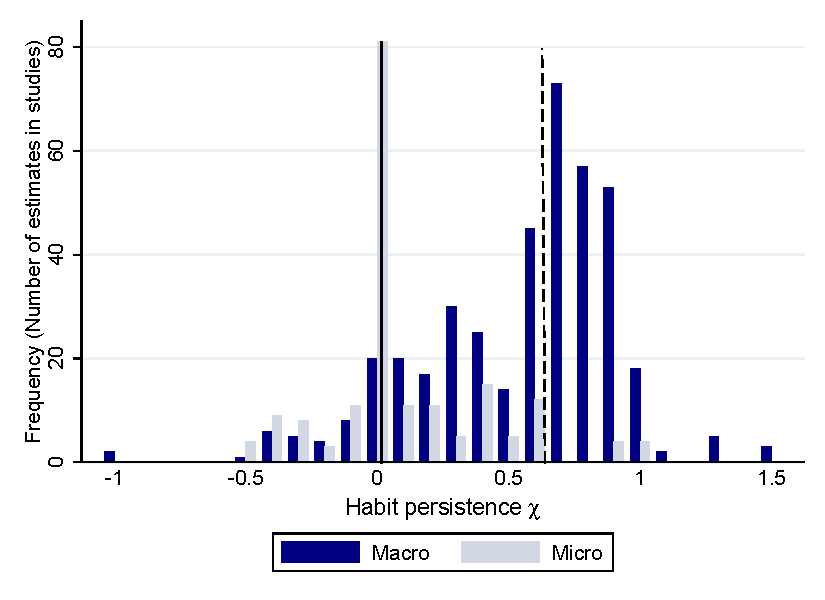
\includegraphics[width=1.0\textwidth]{./Figures/microMacroMetaHistogram}}

    \begin{flushleft}
      \footnotesize Notes: Reproduced from \cite{hrsHabit}, Figure~2. The figure shows the distribution of estimates of habit persistence in studies based on macro and micro data. Solid and dashed lines show the median estimates in micro (0.0) and macro (0.6) studies, respectively.
      \end{flushleft}
\end{figure}

Starting with \cite{cdSmooth}, the macroeconomics, finance, and international economics literatures have concluded that aggregate consumption exhibits `excess smoothness' compared to the benchmark \cite{hallRandomWalk} random walk model of consumption.\footnote{In finance, early references are \cite{abel:aerhabits} and \cite{constantinidesHabits}; in international economics, \cite{gru04}.}  For a standard measure of excess smoothness $\chi$ (defined more precisely below), Figure~\ref{microMacroMetaHistogram} shows that studies using aggregate data estimate that $\chi=0.6$ on average.\footnote{Figure~\ref{microMacroMetaHistogram} is reproduced from a recent comprehensive meta-analysis of 597 published estimates by \cite{hrsHabit}.} A careful reading of the literature suggests that the coefficient is higher, perhaps 0.75, in papers where the data are better measured.

In contrast, parallel work using household-level data rejects the existence of any meaningful degree of excess smoothness.  The modal estimate of the micro literature is $\chi$ of 0; the mean estimate is about 0.1.\footnote{For examples of such studies on aggregate data, see results and references in \cite{fuhrer:habits} or \cite{cee:habits}. For micro data, \cite{dynanHabits} is the best-known study; many others are reported in \cite{hrsHabit}.}

We add a simple (and tractable) information friction to an existing benchmark `microfounded' macro model, and show that the modified model can reconcile the micro and macro empirical facts. As in the standard full-information rational expectations setup, consumers in our framework perfectly (`frictionlessly') perceive their own personal circumstances (employment status, wage rate, wealth, etc). However, information about \textit{macroeconomic} quantities (e.g., aggregate productivity growth) arrives only occasionally (as in the Calvo model of firms' price updating), so that households' macroeconomic expectations are ``sticky,'' as in \cite{mrSlumps} and~\cite{carroll:epidemicinflQJE}. We calculate that our proposed degree of (macro) inattention has negligible utility costs because aggregate shocks are small compared to idiosyncratic shocks.

Aggregate consumption sluggishness \textit{a la} \cite{cdSmooth} arises as follows.  A household whose beliefs about the aggregate economy are out of date will behave in the ways that would have been macroeconomically appropriate (for the consumer's currently observed level of wealth, etc) at the time of their last perception of macroeconomic circumstances.  The lag in perception generates a lag in the response of aggregate spending to aggregate developments; the amount of sluggishness will depend on the frequency with which consumers update.  When our model's updating frequency is calibrated to match estimates of the degree of inattention for other aggregate variables (e.g., inflation) using direct expectations data from surveys of households, the model's implications for the persistence in aggregate consumption growth match the estimates of the `excess smoothness' in the macro literature. 

Despite generating appropriate aggregate smoothness, when estimated on simulated \emph{individual} data (corresponding to microeconomic evidence), regressions in the spirit of  \cite{dynanHabits} (the seminal paper in the micro `excess smoothness' literature) reproduce her finding that at the level of individual households, consumption growth has little predictability at the quarterly frequency -- \cite{dynanHabits}'s regressions typically get $\bar{R}^{2}$'s of about 0.01, and her largest reported value is 0.02, in the ballpark of the corresponding estimates generated by our model.\footnote{\hyperlink{Excess-Sensitivity}{Below} we explain why the \cite{hrsHabit} findings, and our model, are not in substantial conflict with the `excess sensitivity' literature---indeed, our model can explain some puzzles in that literature.}
 
Because our model is formulated as a deviation from a maximizing model, we can calculate explicit utility costs of that deviation, which are small because the comparatively small size of the aggregate shocks means that neglecting them temporarily causes only small and temporary errors in the level of consumption.  Consistent with a theme in the literature all the way back to \cite{ayNearRational}, we find that the utility penalty from these small errors is small, so that our consumers would be willing to pay very little for even perpetually perfect information about macroeconomic conditions.

There are many ways besides ours in which information can be imperfect.  But the review of the literature in our next section shows that the alternative imperfect information frameworks that have been proposed to explain excess smoothness are inconsistent with first-order facts from the micro or the macro literatures (sometimes both).

After the literature review, we begin explaining our ideas with a `toy model' (section~\ref{sec:Quadratic}) in which the key mechanisms can be derived analytically, thanks to extreme simplifying assumptions like quadratic utility and constant factor prices.  We next (section \ref{sec:models}) present the full version of our model, which abides by the more realistic assumptions (CRRA utility, aggregate as well as individual shocks, etc) that have become conventional respectively in the micro and macro literatures. After calibrating the model (section~\ref{sec:calibration}), we describe the stylized facts from both the micro and macro literatures that need to be explained by a good microfounded macroeconomic model of consumption, and show that our model robustly reproduces those facts (section \ref{sec:Results}).
We then (section \ref{sec:uCost}) calculate how much a fully informed consumer would be willing to pay at birth to enjoy instantaneous and perfect knowledge of aggregate developments (not much, it turns out).

\section{Background and Literature Review}\label{sec:relation}

\subsection{Imperfect Information}
Our approach is related to extensive work on other forms of information frictions. These frictions include `noisy information' (cf \cite{pischkeMicroMacro}); costly information processing, as in models with rational inattention (cf \cite{simsInattention}); and models of bounded rationality (cf \cite{gabaixSparsityQJE}).

In rational inattention models, agents have a limited ability to pay attention and allocate that scarce resource optimally. Early work by \cite{reis:inattentive} showed explicitly how rational inattention could lead to excess consumption smoothness.
\cite{mw09:RI} built on that work, and more recently \cite{mackWiedREStud15} study a DSGE model with inattentive consumers and firms using a simple New Keynesian framework in which they replace all sources of slow adjustment (habit formation, Calvo pricing, and wage setting frictions) with rational inattention.  Their setup with rational inattention can match the sluggish responses observed in aggregate data, in response both to monetary policy shocks and to technology shocks. A new paper by \cite{LuoRinGE} studies implications of rational inattention for the dynamics and cross-sectional dispersion of consumption and wealth in a general equilibrium model with CARA utility.

A challenge to the rational inattention approach has been the complexity of solving models that aim to work out the full implications of rational inattention in contexts where the models that match the microeconomic evidence are already formidably mathematically and computationally complex (see below for why this complexity is necessary to match first-order micro consumption facts).  The consumption literature on rational inattention has therefore had to adopt simplifying assumptions about the utility function like quadratic (\cite{simsInattention}, section~6; \cite{luo:inatC}) or CARA (\cite{LuoRinGE}; \cite{reis:inattentive}), or a highly stylized setup of idiosyncratic and aggregate income shocks.\footnote{\cite{sims_beyondLQ} considers a 2-period consumption--saving model with log utility. Otherwise, to our knowledge, the only paper that employs the CRRA utility to solve a consumption--saving problem under rational inattention is \cite{tutino_RIconsumption}. Her contribution is mainly methodological, as her setup is quite stylized (e.g., an i.i.d.\ income process).  It would be interesting to extend her work to a more realistic setup (with permanent/persistent income shocks) and study quantitative implications of rational inattention in a model with both idiosyncratic and aggregate income components.}

As a compromise, %
\cite{gabaixSparsityQJE} has recently proposed a framework that is much simpler than the full rational inattention framework of \cite{simsInattention}, but aims to capture much of its essence.  This approach is relatively new, and while it does promise to be more tractable than the full-bore Simsian framework, even the simplified Gabaix approach would be difficult to embed in a model with a standard treatment of transitory and persistent income shocks, precautionary motives, liquidity constraints, and other complexities entailed in modern models of microeconomic consumption decisions.\footnote{\cite{gabaixSparsityQJE} proposes a framework in which consumers perceive a simplified version of the world because there is a cost to paying attention.  The existence of a fixed cost of paying attention means that beliefs are not updated continuously but episodically, and the framework generates dynamics that, when aggregated, resemble partial adjustment dynamics.  It is beyond the scope of this paper (and would be an interesting project in itself) to determine how this framework would apply in a context like ours, where there are four distinct kinds of shocks (aggregate and idiosyncratic, transitory and permanent), each with very different rewards to attention.}
 .

 It would be similarly challenging to determine how to apply the approaches of \cite{woodfordImperfect} or \cite{msInertiaAER} to our question.\footnote{Arguably, our Calvo-style updating is not too different from what one might get in a suitably adapted version of the \cite{msInertiaAER} model.}

Finally, even for a perfectly attentive consumer, information itself can be imperfect.  The seminal work contemplating this possibility was by \cite{muthOptimal}, whose most direct descendant in the consumption literature is \cite{pischkeMicroMacro} (building on \cite{lucas:imperfectInfo}; see also \cite{ludvigson&michaelides:excesses}).  The idea is that perfectly attentive consumers face a signal extraction problem in determining whether a shock to their income is transitory or permanent.  When a permanent shock occurs, the immediate adjustment to the shock is only partial, since agents' best guess is that the shock is partly transitory and partly permanent.   With the right calibration, such a model could in principle explain any amount of excess smoothness.  But \hyperlink{MuthLucasPischke}{we argue in section}~\ref{sec:Comparisons} that when a model of this kind is calibrated to the actual empirical data, it generates far less smoothness than exhibited in the data.

\subsection{Microfoundations}

No review of the empirical literature on smoothness is needed; \cite{hrsHabit} have done an admirable job.

As for matching ``first-order'' micro facts, a large empirical literature over the last several decades has documented the importance of modeling precautionary saving behavior under uncertainty. For example, in micro data there is incontrovertible evidence---most recently from millions of datapoints from the Norwegian population registry examined by \cite{fhnMPC}---that the consumption function is not linear with respect to wealth.\footnote{More empirical evidence that households that are in some way `constrained' (e.g., have low liquid assets, low income or low credit scores) have large marginal propensities to consume, especially in newer papers, includes: \cite{jpsTax}, \cite{aslCredit}, \cite{bppInequality}, \cite{kvwWealthyH2m}, \cite{jappelliPistaferri_FPMPC}, \cite{parker25million} and \cite{aydinCresponse}.}  It is concave, as the general theory says it should be (\cite{carroll&kimball:concavity}), and this concavity matters greatly for matching the main micro facts.  In addition, there is also nothing that looks  either like the Reis model's prediction that there will be extended periods in which consumption does not change at all, or its prediction that there will be occasional periods in which consumption moves a lot (at dates of adjustment) and then remains anchored at that newer level for another extended period (a similar result holds in the rational-inattention setup of \cite{tutino_RIconsumption}).  This critique applies generically to models that incorporate a convex cost of adjustment---whether to the consumer's stock of information (\cite{reis:inattentive}) or to the level of consumption as in \cite{chettySzeidl:cCommitmentsEcta}.  All such models imply counterfactually `jerky' behavior of spending at the microeconomic level.\footnote{This pattern {\it does} match consumers' purchases of durable goods like automobiles; but the `excess smoothness' facts hold as strongly for aggregate nondurables as for durable goods.  The fixed-adjustment-cost framework matches many other economic decisions well---for instance, individual investors adjust their portfolios sporadically even though the prices of many assets experience large fluctuations at high frequency---and \cite{alvarezGuisoLippi:DurCons} find ``a robust pattern consistent with the assumption that a component of adjustment costs is information gathering'' (p.~2273).}

To better match the micro data, we use the now-conventional microeconomic formulation in which utility takes the Constant Relative Risk Aversion form and uncertainty is calibrated to match micro estimates.  Our assumption that consumers can perfectly observe the idiosyncratic components of their income allows us to use essentially the same solution methods as in the large recent literature exploring models of this kind.
Implementing the state of the art in the micro literature adds a great deal of complexity and precludes a closed form solution for consumption like the one used by Reis. The payoff is that the model is quantitatively plausible enough that, for example, it might actually be usable by policymakers who wanted to assess the likely aggregate dynamics entailed by specific alternative fiscal policy options.

Finally, there is an interesting and growing literature that uses expectations data from surveys in an attempt to directly measure sluggishness in expectations dynamics.
For example, \cite{coibGor:AER15} find that the implied degree of information rigidity in inflation expectations is high, with an average duration of six to seven months between information updates. \cite{fuhrer:JME17} and \cite{fuhrerIntrinsicPersistence} find that even for professional forecasters, forecast revisions are explainable using lagged information, which would not be the case under perfect information processing.  These empirical results are consonant with the spirit of our exercise.

\section{A Quadratic Utility `Toy Model'}\label{sec:Quadratic}

Here we briefly introduce concepts and notation, and motivate the key result using a simple framework, the classic \cite{hallRandomWalk} random walk model, with time separable quadratic utility and geometric discounting by factor $\beta$.  Overall wealth $\mathbf{o}$ (the sum of human and nonhuman wealth) evolves according to the dynamic budget constraint
\begin{eqnarray}
  \mathbf{o}_{t+1} & = & (\mathbf{o}_{t}-\mathbf{c}_{t})\mathsf{R}+\zeta_{t+1}, \label{eq:zAccum}
\end{eqnarray}
 where $\mathsf{R}=(1+\mathsf{r})$ is the interest factor, $\zeta_{t+1}$ is a shock to (total) wealth, and $\mathbf{c}$ is the level of consumption.

With no informational frictions, the usual derivations lead to the standard Euler equation:
\begin{eqnarray*}
  {\mathrm{u}}^{\prime}(\mathbf{c}_{t}) & = & \mathsf{R}\beta \Ex_{t}\big[{\mathrm{u}}^{\prime}(\mathbf{c}_{t+1})\big], \label{eq:QuadEuler}
\end{eqnarray*}
 where $\Ex_{t}$ denotes an assumption of instantaneous perfect frictionless updating of all information. Quadratic ${\mathrm{u}}$ and $\mathsf{R} \beta=1$ imply Hall's random walk proposition:
\begin{eqnarray*}
  \Delta \mathbf{c}_{t+1} & = & \varepsilon_{t+1} \label{eq:dCQuad}.
\end{eqnarray*}
 Consumers spend
\begin{eqnarray*}
  \mathbf{c}_{t} & = & (\mathsf{r}/\mathsf{R}) \mathbf{o}_{t}, \label{eq:cquad}
\end{eqnarray*}
because this is exactly the amount that maintains expected wealth unchanged:
\begin{eqnarray*}
  \Ex_{t}[\mathbf{o}_{t+1}] & = & (\mathbf{o}_{t}-\mathbf{c}_{t})\mathsf{R} = \mathbf{o}_{t}
.
\end{eqnarray*}

\subsection{Sticky Expectations}

Now suppose consumers update their information about $\mathbf{o}_t$, and therefore their behavior, only occasionally.  A consumer who updates in period $t$ obtains precisely the same information that a consumer in a frictionless model would receive, forms the same expectations, and makes the same choices.  Nonupdaters, however, behave as though their former expectations had actually come true (since by definition they have learned nothing to disconfirm their prior beliefs).  For example, consider a consumer who updates in periods $t$ and $t+n$ but not between.  Designating $\widetilde{\mathbf{o}}$ as the consumer's {\it perception} of wealth:
  \begin{eqnarray*}
\widetilde{\mathbf{o}}_{t+j} & \equiv & \Ex_{t}[\mathbf{o}_{t+j}] = \mathbf{o}_{t} \qquad \text{for }  1\le j < n,
\end{eqnarray*}
  the consumer spends according to perceived wealth so that
  \begin{eqnarray*}
\mathbf{c}_{t+j} & = & (\mathsf{r}/\mathsf{R})\widetilde{\mathbf{o}}_{t+j} = (\mathsf{r}/\mathsf{R})     \mathbf{o} _{t} = \mathbf{c}_{t} \qquad \text{for }  1\le j < n.
\end{eqnarray*}
The dynamics of actual (as distinct from perceived) wealth are given by \eqref{eq:zAccum},
\begin{eqnarray*}
 \mathbf{o}_{t+n} & = & \mathbf{o}_{t}+\underbrace{\sum_{s=1}^{n} \mathsf{R}^{n-s}\zeta_{t+s}}_{\equiv\,\Delta^{n} \mathbf{o}_{t+n}},
\end{eqnarray*}
 so for a consumer who updates in periods $t$ and $t+n$ but not between, the change in consumption is
\begin{eqnarray*}
         \mathbf{c}_{t+n}-\mathbf{c}_{t}  & = & (\mathsf{r}/\mathsf{R})\Delta^{n}\mathbf{o}_{t+n},
\end{eqnarray*}
  where $\Delta^{n}\mathbf{o}_{t+n}$ is white noise because it is a weighted sum of the white noise errors $\zeta$.  Thus, consumption follows a random walk across updating periods; consumers who were only observed during their updating periods would never be seen to deviate from the predictions of \cite{hallRandomWalk}.

\subsection{Aggregation}

The economy is populated by consumers indexed by $i$, distributed uniformly along the unit interval.  Aggregate (or equivalently, per capita) consumption is:
\begin{eqnarray*}
        \mathbf{C}_{t} & = & \int_{0}^{1} \mathbf{c}_{t,i}\,\text{d}i
\end{eqnarray*}
 
Whether the consumer at location $i$ updates in period $t$ is determined by the realization of the binary random variable $\pi_{t,i}$, which takes the value 1 if consumer $i$ updates in period $t$ and 0 otherwise.  Each period's updaters are chosen randomly such that a constant proportion $\Pi$ update in each period:
\begin{eqnarray*}
   \Ex[\pi_{t+1,i}] &= & \Pi \qquad \forall\,t \text{ and } i,
\\ \int_{0}^{1} \pi_{t,i}\,\text{d}i & = & \Pi \qquad \forall\,t
\end{eqnarray*}

Aggregate consumption is the population-weighted average of per-capita consumption of updaters $\mathbf{C}^{\pi}$ and nonupdaters $\mathbf{C}^{\cancel{\pi}}$:
\begin{eqnarray}
 \mathbf{C}_{t+1} & = & \Pi \mathbf{C}^{{\pi}}_{t+1}+(1-\Pi) \underbrace{\mathbf{C}^{\cancel{{\pi}}}_{t+1}}_{=\,\mathbf{C}_{t}}, \label{eq:Ctp1}
\end{eqnarray}
where per-capita consumption $\mathbf{C}^{\cancel{{\pi}}}_{t+1}=\mathbf{C}_{t}$ because the
nonupdaters at time $t+1$ are a random subset of the population at time $t$.
The first difference of \eqref{eq:Ctp1} yields:
\begin{eqnarray*}
  \Delta \mathbf{C}_{t+1} & = &  (1-\Pi) \Delta \mathbf{C}_{t} + \underbrace{\Pi \Delta \mathbf{C}^{{\pi}}_{t+1}}_{\equiv\,\varepsilon_{t+1}}, \label{eq:deltac} \label{eq:dCQuadStickyApprox}
\end{eqnarray*}
and online Appendix~\ref{appendix:QuadCDyn} shows that $\varepsilon_{t+1}$ is approximately mean zero. Thus, in the quadratic utility framework the serial correlation of aggregate per-capita consumption changes is an approximate measure of the proportion of nonupdaters.

This is the mechanism behind the exercises presented in section \ref{sec:Results}.  While the details of the informational friction are different in the more realistic model we present in section \ref{sec:models}, the same logic and quantitative result hold: the serial correlation of consumption growth approximately equals the proportion of nonupdaters.

Note further that the model does {\it not} introduce any explicit reason that consumption growth should be related to the predictable component of income growth {\it a la} \cite{cmModel}.  In a regression of consumption growth on the predictable component of income growth (and nothing else), the coefficient on income growth would entirely derive from whatever correlation predictable income growth might have with lagged consumption growth.  This is the pattern we will find below, in both our theoretical and empirical work.

\section{Realistic Model}
\label{sec:models}

One of the lessons of the consumption literature after \cite{hallRandomWalk} is that his simplifying assumptions (quadratic utility, perfect capital markets, $\mathsf{R}\beta=1$) are far from innocuous; more plausible assumptions can lead to very different conclusions.  In particular, a host of persuasive theoretical and empirical considerations has led to the now-standard assumption of constant relative risk aversion utility, ${\mathrm{u}}(\mathbf{c})=\mathbf{c}^{1-\rho}/(1-\rho).$ But when utility is not quadratic, solution of the model requires specification of the exact stochastic structure of the income and transition processes.

Below, we present a model that will be used to simulate the economy under frictionless and sticky expectations.  We specify a small open economy (or partial equilibrium) model with a rich and empirically realistic calibration of idiosyncratic and aggregate risk but exogenous interest rates and wages. In the online appendix, we present two alternative closed economy (general equilibrium) models, along with simulation results analogous to those of section \ref{sec:Results}, replicating our findings in other settings.\footnote{In online Appendix \ref{sec:HADSGE}, we extend the SOE model to a heterogeneous agents dynamic stochastic general equilibrium (HA-DSGE) model that endogenizes factor returns at the cost of considerably more computation, which gives results substantially the same as the SOE model.  Online Appendix \ref{sec:RepAgent} presents a model that abstracts from idiosyncratic income risk (essentially, setting $\sigma^{2}_{\psi}=\sigma^{2}_{\theta}=0$), and which produces results similar to those of our `realistic' models.  The simplification enables general equilibrium analysis at a small fraction of the computational cost. However, it is neither a representative agent model---the distribution of beliefs must be tracked---nor a respectable heterogeneous agents model, which may reduce its appeal to both audiences.}

In our model, a continuum of agents care about expected lifetime utility derived from CRRA preferences over a unitary consumption good; they geometrically discount future utility flows by discount factor $\beta$.  Agents inelastically supply one unit of labor, and their only decision in each period $t$ is how to divide their market resources $\mathbf{m}$ between consumption $\mathbf{c}$ and saving in a single asset $\mathbf{a}$.  We assume agents are \cite{blanchardFinite} ``perpetual youth'' consumers: They have a constant probability of death $\mathrm{d}$ between periods, and upon death they are are immediately replaced, while their assets are distributed among surviving households in proportion to the recipient's wealth.

\subsection{Output, Income, and Productivity}

Output is produced by a Cobb--Douglas technology using capital $\mathbf{K}_t$ and (effective) labor $\mathbf{L}_t$; capital depreciates at rate $\delta$ immediately after producing output, leaving portion $(1-\delta)$ intact, and as usual the effectiveness of labor depends on the level of aggregate labor productivity.  We consider a small open economy with perfect international capital mobility, so that the returns to capital and labor $\mathsf{r}_t$ and $\mathsf{W}_t$ are exogenously determined (at constant values $\mathsf{r}$ and $\mathsf{W}$); this permits a partial equilibrium analysis using only the solution to the individual households' problem.\footnote{See the online appendix for model variants with endogenous factor prices.}

We represent both aggregate and idiosyncratic productivity levels as having both transitory and permanent components.  Large literatures have found that this representation is difficult to improve upon much in either context, and the simplicity of this description yields considerable benefits both in the tractability of the model, and in making its mechanics as easy to understand as possible.

In more detail, aggregate permanent labor productivity $P_t$ grows by factor $\Phi_t$, subject to mean one iid aggregate permanent shocks $\Psi_t$, so the aggregate productivity state evolves according to a finite Markov chain:
\begin{equation}
{P}_{t+1} = \Phi_{t+1} {P}_{t}\Psi_{t+1}, \text{ where} \qquad\text{Prob}[\Phi_{t+1}=\Phi_k | \Phi_t = \Phi_j] = \Xi_{j,k},   \label{eq:AggRandWalk}
\end{equation}
where $j$ and $k$ index the states. The productivity growth factor $\Phi_t$ follows a bounded random walk, as in (for example) \cite{edge2007Learning}, which is part of a literature whose aim is to capture in a simple statistical way the fact that underlying rates of productivity growth seem to vary substantially over time (e.g., fast in the 1950s, slow in the 1970s and 1980s, moderate in the 1990s, and so on; see also \cite{jorgenson:ProductivityGrowthResurgence}).\footnote{We capture the process by discretizing the range of productivity growth rates within our bounds, and calibrate the Markov transition probability matrix $\Xi$ so that the statistical properties of productivity growth rates exhibited by our process match the corresponding properties measured in U.S.\ data since the 1950s.}  We introduce these slow-moving productivity growth rates not just for realism, but also because we need to perform simulated exercises analogous to those of \cite{cmModel} on empirical data, in which consumption growth is regressed on the component of income growth that was predictable using data lagged several quarters.  We therefore need a model in which there {\it is} some predictability in income growth several quarters in the future.

The transitory component of productivity in any period is represented by a mean-one variable $\Theta_t$, so the overall level of aggregate productivity in a given period is $P_{t}\Theta_{t}$.

Similarly, each household has an idiosyncratic labor productivity level $p_{t,i}$, which (conditional on survival) evolves according to:
\begin{equation}
p_{t+1,i} = p_{t,i} \psi_{t+1,i},  \label{eq:IndRandWalk}
\end{equation}
and like their aggregate counterparts, idiosyncratic permanent productivity shocks are mean
one iid ($\Ex_{t}[\psi_{t+n,i}]=\Ex_{t}[\Psi_{t+n}]= 1~\forall ~n>0$).
Total labor productivity for the individual is determined by the interaction of transitory idiosyncratic
($\theta$), transitory aggregate ($\Theta$), permanent idiosyncratic $({p})$, and permanent aggregate
$({P})$ factors.  When the household supplies one unit of labor, effective labor is:
\begin{eqnarray}
  \label{eq:ell}
   \pmb{\ell}_{t,i} & = & \underbrace{\theta_{t,i}\Theta_{t}}_{\equiv\,\pmb{\theta}_{t,i}}\underbrace{{p}_{t,i} {P}_{t}}_{\equiv\,\pmb{p}_{t,i}}.
\end{eqnarray}
  Here, $\theta$ can be thought of as reflecting, for example, individual unemployment spells, while $\Theta$ captures, e.g., disruptions in output due to bad weather.  Just like permanent shocks, transitory shocks are mean one and iid, $\Ex_{t}[\theta_{t+n,i}]=\Ex_{t}[\Theta_{t+n}]=1~\forall~n>0$.  { The idiosyncratic transitory shock has a minimum possible value of 0 (corresponding to an unemployment spell) which occurs with a small finite probability $\wp$.  This has the effect of imposing a `natural borrowing constraint' (cf.\ \cite{zeldesStochastic}) at zero.}{}

\subsection{Perceptions and Behavior}

For understanding the decisions of an individual consumer in a frictionless (i.e.\ perfect information) world the aggregate and idiosyncratic transitory shocks can be combined into a single overall transitory shock indicated by the boldface $\pmb{\theta}$, and the aggregate and idiosyncratic levels of permanent income can be combined as $\pmb{p}$ (likewise, the combined permanent shock is boldface $\pmb{\psi}_{t,i}\equiv \psi_{t,i} \Psi_{t}$).

All households (frictionless and sticky-expectations alike) in our models always correctly observe the \textit{level} of all household-specific variables---they are able to read their bank statement and paycheck. As will be shown below, frictionless consumers' optimal behavior depends on the {\it ratios} of those household-specific variables to permanent productivity $\pmb{p}$.  That is, for some state variable $\textbf{x}$ (like market wealth), the optimal choice for the frictionless consumer would depend on ${x} \equiv \mathbf{x}/{\pmb{p}}$, where our definition of nonboldface ${x}$ reflects our notational convention that when a level variable has been normalized by the corresponding measure of productivity, it loses its boldness.  The same applies for aggregate variables, e.g.\ ${X} \equiv \mathbf{X}/{P}$.

One reason we assume that both frictionless and sticky-expectations consumers can perceive the idiosyncratic components of their income (the $p$ and $\theta$) is that this is the assumption made by almost all of the `modern' literature, and therefore makes our paper's results easily comparable with that literature.

But the assumption can be defended on its own terms; it is consistent with evidence from a number of sources.

First, there are at least some shocks whose transitory nature is impossible to misperceive; the best example is lottery winnings in Norway, see again \cite{fhnMPC}.  The consumption responses to those shocks resemble the responses measured in the previous literature to shocks that economists presumed that consumers knew to be transitory.  If consumers respond to such shocks in ways similar to their responses to unambiguously transitory shocks like lottery winnings, that would seem to support the proposition that consumers correctly perceive as transitory those other shocks that economists have presumed consumers identified as transitory.

Second, one reason to believe that perception of the idiosyncratic permanent shocks is not difficult comes from \cite{lmpPermShocks}, who show that a large proportion of permanent shocks to income occur at the times of job transitions (mostly movements from one job to another).  It would be hard to believe that consumers switching jobs were not acutely aware of the difference between the incomes yielded by those two jobs.

Earlier work by \cite{pistaferriSuperior} developed a method for decomposing income shocks into permanent and transitory components.  He finds that data from a survey in which consumers are explicitly asked about their income expectations provides a powerful tool to estimate the magnitude of permanent versus transitory shocks; relatedly, \cite{gsInferring} find that consumption choices provide important information about subsequent income movements.

More direct and more recent evidence comes from \cite{kmpIncomeExpectations}.  Using data from the New York Fed's Survey of Consumer Expectations (SCE), they find that on average, the difference between four-month-ahead realizations of household income and four-month-ahead expectations is near zero and the average error is only 0.5 percent. \cite{kmpIncomeExpectations} explicitly interpret their evidence from the survey as suggesting that consumers have accurate perceptions of the permanent and transitory components of their income.

A final bit of evidence comes from metadata associated with the \textit{Survey of Consumer Finances}, which asks a question designed to elicit consumers' perceptions of their permanent (``usual'') income.  A well-known fact in among survey methodologists is that the speed and ease with which consumers answer a question is an indicator of the extent to which they have a clear understanding of the question and are confident in their answer.  The SCF question designed to elicit consumers perceptions of their permanent income is an example of such a question: Consumers answer quickly and easily and do not seem to exhibit any confusion about what they are being asked (\cite{kennickellPermanent}).

In contrast, we are aware of no corresponding evidence that consumers are well informed about aggregate income (especially at high frequencies). %
 This is why we have assumed that the inattention that drives our model applies only to perceptions of the (tiny) contribution that aggregate productivity state variables $\{P_t,\Phi_t\}$ make to consumers' overall income.

We denote consumer $i$'s \textit{perceptions} about the aggregate state $\{\widetilde{P}_{t,i},\widetilde{\Phi}_{t,i}\}$.  Our key behavioral assumption is twofold:
\begin{enumerate}
\item Households always act \textit{as if} their perception of the aggregate state $\{\widetilde{P}_{t,i},\widetilde{\Phi}_{t,i}\}$ were the true aggregate state $\{P_t,\Phi_t\}$.

\item As in the `toy model', households form their perception of the aggregate state according to the \textit{expectation} of today's state that corresponds to the information they had the last time they observed the aggregate state.
\end{enumerate}
Given the assumption that the productivity growth factor $\Phi_t$ follows a random walk,
the second part of the behavioral assumption says that an agent who last observed the true
aggregate state $n$ periods ago perceives:
\begin{equation}\label{eq:PLevBelief}
\{\widetilde{P}_{t,i},\widetilde{\Phi}_{t,i}\} = \Ex_{t-n}\big[\{P_t,\Phi_t\} \big| \{P_{t-n},\Phi_{t-n}\}\big] = \left\{\Phi_{t-n}^{n} P_{t-n},\Phi_{t-n}\right\}.
\end{equation}
That is, our assumed random walk in productivity growth means that the household believes that the aggregate productivity factor has remained at $\Phi_{t-n}$ for the past $n$ periods, and remains there today.\footnote{Because of the boundedness of the random walk in productivity growth, this does not hold exactly when the productivity growth state is in the bottommost or topmost Markov bin; we neglect the small error entailed by this fact.}  For households who observed the true aggregate state this period, $n=0$ and thus \eqref{eq:PLevBelief} says that $\{\widetilde{P}_{t,i},\widetilde{\Phi}_{t,i}\} = \{P_t,\Phi_t\}$.

Given their perception of the aggregate level of productivity, the household perceives that their overall permanent productivity level to be $\widetilde{\pmb{p}}_{t,i} = p_{t,i} \widetilde{P}_{t,i}$.

The behavior of a `sticky expectations' consumer thus differs from that of a frictionless consumer only to the extent that the `sticky expectations' consumer's perception of aggregate productivity is out of date.

When a household's perception of productivity $\widetilde{\pmb{p}}$ differs from actual productivity, we denote the perceived ratio as, e.g., $\widetilde{x} \equiv \mathbf{x}/\widetilde{\pmb{p}} = \mathbf{x}/({p}\widetilde{P})$ where the last equality reflects our assumption that the household perceives the idiosyncratic component of their productivity ${p}$ without error.

\subsection{Transition Dynamics}

Infinitely-lived households with a productivity process like \eqref{eq:IndRandWalk} would generate a nonergodic distribution of idiosyncratic productivity---as individuals accumulated ever more shocks to their permanent productivities, those productivities would spread out indefinitely across the population with time. To avoid this inconvenience, we make the \cite{blanchardFinite} assumption: Each consumer faces a constant probability of mortality of $\mathrm{d}$. We track death events using a binary indicator:
\begin{equation*}
\mathsf{d}_{t+1,i} =
  \begin{cases}
    0 & \text{if consumer at location $i$ survives from time $t$ to $t+1$}
\\    1 & \text{if consumer at location $i$ dies between $t$ and $t+1$}.
  \end{cases}
\end{equation*}
We refer to this henceforth as a `replacement' event, since the consumer who dies is replaced by an unrelated newborn who happens to inhabit the same location on the number line.  The {\it ex ante} probability of death is identical for each consumer, so that the aggregate mass of consumers who are replaced is time invariant at $\mathrm{d} = \int_{0}^{1} \mathsf{d}_{t,i}\,di$ (again using the notation that capital letters represent aggregate values).

\begin{equation*}  
{p}_{t+1,i} =
  \begin{cases}
       {p}_{t,i} \psi_{t+1,i} & \text{if } \mathsf{d}_{t+1,i} = 0 \\
    1 & \text{if } \mathsf{d}_{t+1,i} = 1. \\
  \end{cases}
\end{equation*}
 There is no relationship between successive persons at the same location on the number line (this is not a dynastic model).

Along with its productivity level, the household's primary state variable when the consumption decision is made is the level of market resources $\mathbf{m}_{t,i}$, which captures both current period labor income $\mathbf{y}_{t,i}$ (the wage rate times the household's effective labor supply) and the resources that come from the agent's capital stock $\mathbf{k}_{t,i}$ (the value of the capital itself plus the capital income it yields):
\begin{equation}
  \mathbf{m}_{t,i} = \underbrace{{\bf \mathsf{W}}_{t} \pmb{\ell}_{t,i}}_{\equiv\,\mathbf{y}_{t,i}} + \underbrace{{\mathscr{R}}_t}_{1-\delta+\mathsf{r}_{t}} \mathbf{k}_{t,i}.
\label{eq:mDef}
\end{equation}
 The transition process for $\mathbf{m}$ is broken up, for convenience
of analysis, into three steps.  `Assets' at the end of the period are
market resources minus consumption:
\begin{eqnarray}
   \mathbf{a}_{t,i} & = & \mathbf{m}_{t,i}-\mathbf{c}_{t,i}. \label{eq:aDef}
\end{eqnarray}
 Next period's capital is determined from this period's assets via:
\begin{eqnarray}
\mathbf{k}_{t+1,i} & = & \mathsf{d}_{t+1,i} \cdot 0+ (1 - \mathsf{d}_{t+1,i})\mathbf{a}_{t,i} \big/(1-\mathrm{d}) \label{eq:ktp1icompact}
\end{eqnarray}
where the first term represents `newborns' having zero assets, and the second term's division of $\mathbf{a}$ by the survival probability $(1-\mathrm{d})$ reflects returns to survivors from the Blanchardian insurance scheme.

\subsection{Aggregation}

The foregoing assumptions permit straightforward aggregation of individual-level variables.  Aggregate capital is the population integral of \eqref{eq:ktp1icompact}:
\begin{equation}
\mathbf{K}_{t} = \int_{0}^{1} \mathbf{k}_{t,i}\,\text{d}i = \int_{0}^{1} \big((1 - \mathsf{d}_{t,i})\mathbf{a}_{t-1,i} \big/(1-\mathrm{d})\, \big)\,\text{d}i = \int_{0}^{1} \mathbf{a}_{t-1,i}\,\text{d}i = \mathbf{A}_{t-1}.   \label{eq:Ktp1}
\end{equation}
 The third equality holds because $(1-\mathrm{d})^{-1}\int_{0}^{1}(1-\mathsf{d}_{t,i})\,\text{d}i = 1$
since $\mathsf{d}_{t,i}$ is independent of $\mathbf{a}_{t-1,i}$.
Because $\int_{0}^{1} \theta_{t,i} = \int_{0}^{1} {p}_{t,i} = 1,$ aggregate labor supply
is
\begin{eqnarray}
  \label{eq:Lt}
  \mathbf{L}_{t} & = & \int_{0}^{1} \pmb{\ell}_{t,i}\,\text{d}i = \Theta_{t} {P}_{t}.
\end{eqnarray}

Aggregate market resources can be written as per-capita resources of the survivors times their population mass $(1-\mathrm{d})$, plus per-capita resources of the newborns times their population mass $\mathrm{d}$:
\begin{eqnarray}
  \mathbf{M}_{t} & = & \big(\overbrace{\mathbf{A}_{t-1} {\mathscr{R}}_t/(1-\mathrm{d})  + \Theta_{t} {P}_{t}\mathsf{W}}^{\text{per-capita $\mathbf{m}$ for survivors}}\big)(1-\mathrm{d})+\overbrace{\Theta_{t} {P}_{t}\mathsf{W}_t}^{\text{per-capita $\mathbf{m}$ for newborns}} \mathrm{d} \nonumber \\
                       & = & \mathbf{A}_{t-1} {\mathscr{R}}_t + \Theta_{t} P_t \mathsf{W}_t  \label{eq:Mtp1} \\
                       & = & \mathbf{K}_t \mathscr{R}_t + \mathbf{L}_t \mathsf{W}_t. \nonumber
\end{eqnarray}
 

The productivity-normalized version of \eqref{eq:Mtp1} says that
\begin{equation}\label{eq:Mtp1norm}
M_t = A_{t-1} \mathscr{R}_t\big/(\Psi_t \Phi_t) + \Theta_t \mathsf{W}_t.
\end{equation}
We will sometimes refer to the factor $P_t\big/\widetilde{P}_{t,i}$ as the household's `productivity misperception,' the scaling factor between actual and perceived market resources.

\subsection{Model Solution}

Because of the assumption of a small open economy, the frictionless consumer's state variables are simply $(\mathbf{m}_{t,i},p_{t,i},P_t,\Phi_t)$.  As we assume that the sticky expectations consumer behaves according to the decision rules that are optimal for the frictionless consumer but using perceived rather than true values of the state variables, we need only to solve for the frictionless solution.

The household's problem in levels can be written in Bellman form as:\footnote{Subject to definitions \eqref{eq:AggRandWalk}, \eqref{eq:IndRandWalk}, \eqref{eq:ell}, \eqref{eq:mDef}, \eqref{eq:aDef} and \eqref{eq:ktp1icompact}.}
\begin{eqnarray*}
\textbf{v}(\mathbf{m}_{t,i},p_{t,i},P_t,\Phi_t)  & = &  \max_{\mathbf{c}_{t,i}}  \big\{ {\mathrm{u}}(\mathbf{c}_{t,i}) + \beta \Ex_t \big[(1-\mathsf{d}_{t+1,i})\textbf{v}(\mathbf{m}_{t+1,i},p_{t+1,i},P_{t+1},\Phi_{t+1})\big] \big\}. \nonumber
\end{eqnarray*}
Our assumption that the aggregate and idiosyncratic productivity levels both reflect a combination of purely transitory and purely permanent components now permits us to make a transformation that considerably simplifies analysis and solution of the model: When the utility function is in the CRRA class, the problem can be simplified by dividing by $\pmb{p}_{t,i}^{1-\rho} = (p_{t,i}P_t)^{1-\rho}$ while converting to normalized variables as above (e.g., $m_{t,i}=\mathbf{m}_{t,i}/\pmb{p}_{t,i}$).\footnote{This is well understood in the literature; for a full exposition, see, e.g., \cite{BufferStockTheory}.}  This yields the normalized form of the problem, which has only $m_{t,i}$ and $\Phi_t$ as state variables:
\begin{eqnarray}
    \mathrm{v}({m}_{t,i},\Phi_t) & = & \max_{c_{t,i}} ~ \big\{ {\mathrm{u}}(c_{t,i}) + (1-\mathrm{d}) \beta
    \Ex_{t}\big[ (\Phi_{t+1} \pmb{\psi}_{t+1,i})^{1-\rho}\mathrm{v}(m_{t+1,i},\Phi_{t+1})\big] \big\}
    \label{eq:scaledv}
\\  & \mbox{s.t.} & \nonumber
\\    a_{t,i}   & = & m_{t,i} - c_{t,i}, \nonumber
\\    k_{t+1,i} & = & a_{t,i} \big/( (1-\mathrm{d}) \Phi_{t+1} \pmb{\psi}_{t+1,i} ),  \nonumber
\\    m_{t+1,i} & = & \mathscr{R} k_{t+1,i} + \mathsf{W} \pmb{\theta}_{t+1,i}.  \nonumber
\end{eqnarray}
 
Defining $\mathsf{R} = \mathscr{R}\big/(1-\mathrm{d})$, the main requirement for this problem to have a useful solution is an impatience condition:\footnote{Other parametric restrictions are also necessary, but for typical parameterizations are not likely to be binding; see \cite{BufferStockTheory} for details.  Note that the relevant interest factor is the within-period productivity of capital $\mathscr{R}$ is the gross return adjusted for both of the influences, $\delta$ and $(1-\mathrm{d})$, that intervene between the amount of assets with which the consumer ends period $t$ and the amount of productive capital owned by a survivor when capital income is received in period $t+1$.  }
\begin{eqnarray*}
  \label{eq:impatience}
  \mathsf{R} \beta  \Ex[ \pmb{\psi}^{-\rho}]  & < & 1.
\end{eqnarray*}
 
Designating the converged normalized consumption function that solves \eqref{eq:scaledv} as
$\mathrm{c}(m,\Phi)$, the level of consumption for the frictionless consumer can be obtained\footnote{Online Appendix~\ref{appendix:Solution}
provides details for numerically solving the model.} from
\begin{eqnarray}
  \label{eq:cFlevel}
   \mathbf{c}_{t,i} & = & \pmb{p}_{t,i} \mathrm{c}(m_{t,i},\Phi_t)  \nonumber
.
\end{eqnarray}
 Because the model is homothetic in $\pmb{p}_{t,i}={p}_{t,i} {P}_{t}$, this can be equivalently written with the un-normalized consumption function $\textbf{c}$ as:
\begin{eqnarray*}
\mathbf{c}_{t,i} & = & \textbf{c}(\mathbf{m}_{t,i}, p_{t,i}, {P}_t, {\Phi}_t).
\end{eqnarray*}

\subsection{Frictionless vs Sticky Expectations}\label{sec:StickySOE}

Following the same notation as in the motivating section \ref{sec:Quadratic}, we define an indicator variable for whether household $i$ updates their perception to the true aggregate state in period $t$:\footnote{For simplicity, newborns begin life with correct beliefs about the aggregate state.  This assumption about newborns' beliefs is numerically inconsequential because the quarterly replacement rate is so low; see section~\ref{sec:calibration} for details.}
\begin{equation*}
\pi_{t,i} =
\begin{cases}
   1 & \text{if consumer $i$ updates in period $t$}
\\ 0 & \text{if consumer $i$ does not update in period $t$}.
\end{cases}
\end{equation*}

The Bernoulli random variable $\pi_{t,i}$ is iid for each household each period, with a probability $\Pi$ of returning 1.  Consistent with \eqref{eq:PLevBelief}, household beliefs about the aggregate state evolve according to:
\begin{equation}\label{eq:PLevBeliefSOE}
\{\widetilde{P}_{t,i},\widetilde{\Phi}_{t,i}\} = \begin{cases}
\{P_t, \Phi_t\} & \text{if } \pi_{t,i} = 1 \\
\{\widetilde{\Phi}_{t-1,i} \widetilde{P}_{t-1,i} , \widetilde{\Phi}_{t-1,i} \} & \text{if } \pi_{t,i} = 0.
\end{cases}
\end{equation}

Under the assumption that consumers treat their belief about the aggregate state as if it were the truth, the relevant inputs for the normalized consumption function $\mathrm{c}(m,\Phi)$ are the household's \textit{perceived} normalized market resources $\widetilde{m}_{t,i} = \mathbf{m}_{t,i}\big/\widetilde{\pmb{p}}_{t,i} = \big(P_t\big/\widetilde{P}_{t,i}\big)m_{t,i}$ and perceived aggregate productivity growth $\widetilde{\Phi}_{t,i}$.  The household chooses the level of consumption by:
\begin{equation*}
   \mathbf{c}_{t,i} = \widetilde{\pmb{p}}_{t,i} \mathrm{c}(\widetilde{m}_{t,i},\widetilde{\Phi}_{t,i}) = \textbf{c}(\mathbf{m}_{t,i}, p_{t,i}, \widetilde{P}_{t,i}, \widetilde{\Phi}_{t,i}). \label{eq:cPerc}
\end{equation*}
 The behavior of the `sticky expectations' consumer converges to that of the frictionless consumer as $\Pi$ approaches 1.

Because households in our model never misperceive the \textit{level} of their own market resources ($\widetilde{\mathbf{m}}_{t,i}=\mathbf{m}_{t,i}$), they can never choose consumption that would violate the budget constraint.  Households observe both their level of income $\mathbf{y}_{t,i}$ and its idiosyncratic components $\theta_{t,i}$ and ${p}_{t,i}$. If they wanted to do so, households could therefore calculate the aggregate component $\Theta_{t}\times {P}_{t}$, which would correspond with the reports of a statistical agency; but they do \textit{not} observe $\Theta_{t}$ and ${P}_{t}$ separately (because, in our model as in reality, statistical agencies do not report these objects).

Our assumption is simply that households with sticky expectations neither perceive nor attempt to extract an estimate of the decomposition of that aggregate state into transitory and permanent components.  Consumers' misperceptions of aggregate permanent income \textit{do} cause them to make systematic errors---but below we present calculations showing that for the value of $\Pi$ that we estimate, those errors have small utility costs.

The utility costs would be a bit smaller if consumers were to perform a certainty-equivalent signal extraction and behaved as though the signal-extracted estimate of the aggregate state is ``truth'' (that is, they ignore the fact that their estimate has an error term), but section~\ref{sec:Comparisons} analyzes the alternative model in which households perform such a signal extraction and shows that the dynamics of aggregate consumption under this assumption do not match the dynamics that are observed in the aggregate data.

\subsubsection{Alternative Beliefs About the Aggregate Income Process}
A model in which households understand that their macroeconomic beliefs are out-of-date due to inattention and prudently change their behavior to account for the extent of their uncertainty at any given moment would be far more computationally costly to solve (adding several additional state variables).  This reflects the fact that the mathematically correct treatment of widening aggregate uncertainty is formidably difficult.  But if the benefits to consumers of keeping track of the consequences of their growing ignorance were large, we might feel that we had no choice but to go down that path.

Consumers' motivation to take account of the widening of their uncertainty as the distance from the last update increases springs from the convexity of marginal utility with respect to larger shocks: Compared to experiencing four shocks of a given size, experiencing one shock that is four times is large is strictly worse.  The magnitude of the benefit to consumers from accounting for correctly for their expanding aggregate uncertainty is related to the \textit{degree} to which the one big shock is worse than the four smaller shocks.

To gauge that magnitude, we conducted an experiment.  In online Appendix~\ref{appendix:AltBelief}, we present a specification in which sticky expectations households optimize under the belief that aggregate shocks only arrive in one in four quarters, but with four times the variance of the quarterly shocks, matching approximately how they will actually \textit{perceive} the arrival of macroeconomic information; the consumption function and main results are virtually identical under these alternate beliefs, which makes us comfortable in not attempting the challenging task of computing the optimal behavior that takes into account the widening uncertainty about the aggregate state as the time since the last update increases.

\subsection{Calibration}\label{sec:calibration}

The full set of parameters is presented in Table~\ref{table:calibration}.  We offer complete discussion of our calibration in online Appendix~\ref{app:Calibration}, but a few aspects warrant comment here.

In the SOE model, we set a much lower value of $\beta$ ($ %
0.97 %
 $) than would be expected given our calibrated return factor (${\mathscr{R}} = 1.015$), resulting in agents with wealth holdings around the median observed in the data.  This reflects the recent literature finding that for purposes of capturing aggregate consumption dynamics it may be more important to match the behvior of the typical consumer rather than the behavior of the typical holder of a dollar of wealth.\footnote{See, for example, \cite{opLiquidH2M}.}  Readers who prefer a calibration matching \textit{mean} observed wealth can consult the online appendix for a closed economy general equilibrium model, in which we show that the main results still hold.

We calibrated the process for trend aggregate productivity growth $\Phi$ to match measured U.S.\ productivity data.  A Markov process with eleven states ranging between $-3.0$ percent and $+3.0$ percent (annual), and in which the state changes on average every two quarters, allowed us to fit both the high frequency autocorrelation evidence cited above and the low-frequency component of productivity growth obtained, e.g., by \cite{sswNAIRU}, Figure~1.9 and \cite{fernald:disappointingRecovery}, Figure~10.

In our calibration, the variance of the idiosyncratic permanent innovations at the quarterly frequency is about 100 times the variance of the aggregate permanent innovations ($4 \times $0.00004 divided by $%
0.012 %
 $).  This is a point worth emphasizing: Idiosyncratic uncertainty is {\it approximately two orders of magnitude larger} than aggregate uncertainty.  While reasonable people could differ a bit from our calibration of either the aggregate or idiosyncratic risk, no plausible calibration of either magnitude will change the fundamental point that the aggregate component of risk is tiny compared to the idiosyncratic component.  This is why assuming that people do not pay close attention to the macroeconomic environment is plausible: It makes a negligible contribution to the total uncertainty they face.

\subsubsection{Small Aggregate Shocks and Consumption Concavity}
A reader who is persuaded of the general importance of precautionary motives and other causes of nonlinearity in the microeconomic consumption function might feel uneasy about our assumption that consumers act in what seems to be a `certainty equivalent' way with respect to aggregate shocks.  The prior paragraph explains why the consequences of this assumption are negligible: Misperception of the level of aggregate productivity is so small that the consumption function is \textit{approximately} linear over the span between the level of consumption that would be correct with full knowledge, and the level of consumption that the consumer actually chooses.  The global concavity of the consumption function (and the curvature of marginal utility), which are important for many other purposes, are of little consequence for errors small enough not to interact meaningfully with that nonlinearity.  The importance of this insight has recently been emphasized by \cite{bmpMITshocks}, who show that assuming that behavior is linear with respect to aggregate shocks has huge benefits for computation of the solution to heterogeneous agent economies, at little cost to microeconomic realism.

We calibrate the probability of updating at $\Pi= %
0.25 %
 $ per quarter, for several reasons.  First, this is the parameter value assumed for the speed of expectations updating by \cite{mrSlumps} in their analysis of the consequences of sticky expectations for inflation.  They argue that an average frequency of updating of once a year is intuitively plausible.  Second, \cite{carroll:epidemicinflQJE} estimates an empirical process for the adjustment process for household inflation expectations in which the point estimate of the corresponding parameter is 0.27 for inflation expectations and 0.32 for unemployment expectations; the similarity of these figures suggests 0.25 is a reasonable benchmark, and provides some insulation against the charge that the model is {\it ad hoc}: It is calibrated in a way that corresponds to estimates of the stickiness of expectations in a fundamentally different context.  Finally, empirical results presented below will also suggest a speed of updating for U.S.\ consumption dynamics of about 0.25 per quarter.

\begin{minipage}{\textwidth}
  \begin{table}
    \centering
    \caption{Calibration}\label{table:calibration}
\begin{tabular}{cd{5}l}  
\\ \toprule  
\multicolumn{3}{c}{\textbf{Macroeconomic Parameters} }  
\\ $\alpha$ & 0.36 & Capital's Share of Income   
\\ $\delta$ & \multicolumn{1}{c}{$1-0.94^{1/4}$} & Depreciation Rate   
\\ $\sigma_{\Theta}^{2}$ & 0.00001 & Variance Aggregate Transitory Shocks 
\\ $\sigma_{\Psi}^{2}$ & 0.00004 & Variance Aggregate Permanent Shocks 
\\ \midrule  
\multicolumn{3}{c}{ \textbf{Steady State of Perfect Foresight DSGE Model} } \  
\\ \multicolumn{3}{c}{ $(\sigma_{\Psi}=\sigma_{\Theta}=\sigma_{\psi}=\sigma_{\theta}=\wp=\mathrm{d}=0$, $\Phi_t = 1)$} \  
\\ ${K}/{K}^{\alpha}$ & 12.0 & SS Capital to Output Ratio  
\\ ${K}$ & 48.55 & SS Capital to Labor Productivity Ratio ($=12^{1/(1-\alpha)}$) 
\\ ${\mathsf{W}}$ &  2.59 & SS Wage Rate ($=(1-\alpha){K}^{\alpha}$) 
\\ ${\mathsf{r}}$ & 0.03 & SS Interest Rate ($=\alpha {K}^{\alpha-1}$) 
\\ ${\mathscr{R}}$ & 1.015& SS Between-Period Return Factor ($=1 - \delta + {\mathsf{r}}$) 
\\ \midrule  
\multicolumn{3}{c}{ \textbf{Preference Parameters} }  
\\ $\rho$ & 2. & Coefficient of Relative Risk Aversion 
\\ $\beta$ &  0.970 & Discount Factor (SOE Model) 
\\ $\Pi$                    & 0.25  & Probability of Updating Expectations (if Sticky) 
\\ \midrule  
\multicolumn{3}{c}{ \textbf{Idiosyncratic Shock Parameters} }  
\\ $\sigma_{\theta}^{2}$    & 0.120     & Variance Idiosyncratic Tran Shocks (=$4 \times$ Annual) 
\\ $\sigma_{\psi}^{2}$      &0.003      & Variance Idiosyncratic Perm Shocks (=$\frac{1}{4} \times$ Annual) 
\\ $\wp$                    & 0.050  & Probability of Unemployment Spell 
\\ $\mathrm{d}$             & 0.005  & Probability of Mortality 
\\ \bottomrule 
 \multicolumn{3}{p{0.95\textwidth}}{ \footnotesize \textbf{Note:} As discussed in online Appendix~\ref{app:Calibration}, we calibrate to the steady state values from a perfect foresight DGSE model.}
\end{tabular}
\end{table}
\end{minipage}

\section{Results}\label{sec:Results}

The calibrated model can now be used to evaluate the effects of sticky expectations on consumption dynamics.  We begin this section with an empirical benchmark on U.S.\ data that will guide our investigation of the implications of the model.  We then demonstrate that simulated data from the sticky expectations models quantitatively and qualitatively reproduces the key patterns of aggregate and idiosyncratic consumption data.

\subsection{U.S.\ Empirical Benchmark}
\label{sec:EmpBenchmark}

The random walk model provides the framework around which both micro and macro consumption literatures have been organized.  Reinterpreted to incorporate CRRA utility and permit time-varying interest rates, the random walk proposition has frequently been formulated as a claim that $\mu=0$ in regressions of the form:
\begin{eqnarray}
  \label{eq:RandomWalkCRRA}
  \Delta \log \mathbf{C}_{t+1} & = & \varsigma+\nu \Ex_{t}[\mathbf{r}_{t+1}]+\mu X_{t}+\epsilon_{t+1},
\end{eqnarray}
where $X_{t}$ is any variable whose value was known to consumers
when the period-$t$ consumption decision was made, and $\epsilon_{t+1}$
is white noise.

For macroeconomic models (including the HA-DSGE setup in online Appendix~\ref{sec:HADSGE}), our simulation analysis\footnote{Readers can confirm these results using the toolkit for solving the model available at the \href{https://github.com/econ-ark/REMARK/tree/master/REMARKs/cAndCwithStickyE}{Econ-ARK/REMARK} resource; the authors can provide particular specifications to produce all claimed results.}
shows that the relationship between the normalized asset stock $A_{t}$ and the expected interest rate $\Ex_{t}[\mathbf{r}_{t+1}]$ is nearly linear, so \eqref{eq:RandomWalkCRRA} can be reformulated with no loss of statistical power as
\begin{eqnarray*}
  \label{eq:RandomWalkAForm}
  \Delta \log \mathbf{C}_{t+1} & = & \varsigma+\alpha A_{t}+\mu X_{t}+\epsilon_{t+1}.
\end{eqnarray*}
This reformulation is convenient because the literatures on precautionary saving and liquidity constraints since at least \cite{zeldes:jpe,zeldesStochastic} have argued that the effects of capital market imperfections can be captured by incorporating a lagged measure of resources like $A_{t}$ in consumption growth regressions.

\cite{cmModel} famously proposed a modification of this model in which a proportion $\eta$ of income goes to rule-of-thumb consumers who spend $C=Y$ in every period.  They argued that $\eta$ can be estimated by incorporating the predictable component of income growth as an additional regressor.  Finally, \cite{dynanHabits} and \cite{som07} show that in standard habit formation models, the size of the habit formation parameter can be captured by including lagged consumption growth as a regressor.  These considerations lead to a benchmark specification of the form:
\begin{eqnarray}
  \label{eq:CGrowBench}
  \Delta \log \mathbf{C}_{t+1} & = & \varsigma+\chi \Delta \log \mathbf{C}_{t}+\eta \Ex_{t}[\Delta \log \mathbf{Y}_{t+1}]+\alpha A_{t}+\epsilon_{t+1}.
\end{eqnarray}

There is an extensive existing literature on aggregate consumption dynamics, but \cite{som07} is the only paper we are aware of that estimates an equation of precisely this form in aggregate data.  He interprets the serial correlation of consumption growth as reflecting habit formation.\footnote{\cite{weber:ruleofthumb} makes a similar point using a different methodology.}  However, Sommer's choice of instruments, estimation methodology, and tests do not correspond precisely to our purposes here, so we have produced our own estimates using U.S.\ data.

\begin{table} \caption{Aggregate Consumption Dynamics in US Data}  \label{table:USCampManVsStickyE}
\centering
\centerline{$\Delta\log\mathbf{C}_{t+1}=\varsigma+\chi\Delta\log\mathbf{C}_t+\eta\Ex_t[\Delta\log\mathbf{Y}_{t+1}]+\alpha A_t+\epsilon_{t+1}$ }
\newsavebox{\CampManBox}  
\sbox{\CampManBox}{  
  \begin{tabular}{d{4}d{4}d{5}cd{4}d{5}}
\toprule
\multicolumn{3}{c}{Measure of Consumption} & OLS &  \multicolumn{1}{c}{2${}^{\text{nd}}$ Stage}  &  \multicolumn{1}{c}{KP $p$-val}
\\ \multicolumn{3}{c}{Independent Variables} & or IV & \multicolumn{1}{c}{$ \bar{R}^{2} $} & \multicolumn{1}{c}{Hansen J $p$ val}
\\ \midrule
\multicolumn{6}{l}{Nondurables and Services }
\\ \multicolumn{1}{c}{$\Delta \log \mathbf{C}_{t} $} & \multicolumn{1}{c}{$\Delta \log \mathbf{Y}_{t+1}$}& \multicolumn{1}{c}{$ A_{t}  $} & & & \\

0.468  & & & OLS & 0.216 & \\
 (0.076)  &  &  & &  &  \\
0.830  & & & IV & 0.278 & 0.222 \\
   (0.098)  &  &  & &  & 0.439 \\
    & 0.587 & & IV & 0.203 & 0.263 \\
   &  (0.110)  &  & &  & 0.319  \\
    &  &     -0.17\text{e$-4$}  & IV & -0.005 & 0.081 \\
   &  &  (     5.71\text{e$-4$})  & & & 0.181  \\
0.618 & 0.305 &     -4.96\text{e$-4$} & IV & 0.304 & 0.415 \\
  (0.159) & (0.161) &  (     2.94\text{e$-4$})  & & & 0.825 \\
  \multicolumn{6}{l}{ Memo: For instruments $\mathbf{Z}_t, \Delta\log\mathbf{C}_{t}=\mathbf{Z}_t \zeta, ~\bar{R}^2= 0.358 $ } \\
 \midrule 
 \multicolumn{6}{l}{ Nondurables } \\
 \multicolumn{1}{c}{$\Delta \log \mathbf{C}_{t} $} & \multicolumn{1}{c}{$\Delta \log \mathbf{Y}_{t+1}$}& \multicolumn{1}{c}{$ A_{t}  $} & & & \\

0.200  & & & OLS & 0.036 & \\
 (0.058)  &  &  & &  &  \\
0.762  & & & IV & 0.083 & 0.504 \\
   (0.284)  &  &  & &  & 0.727 \\
    & 0.849 & & IV & 0.061 & 0.398 \\
   &  (0.357)  &  & &  & 0.731  \\
    &  &      9.09\text{e$-4$}  & IV & 0.008 & 0.118 \\
   &  &  (     9.05\text{e$-4$})  & & & 0.446  \\
0.620 & 0.313 &     -3.25\text{e$-4$} & IV & 0.077 & 0.523 \\
  (0.292) & (0.286) &  (     8.32\text{e$-4$})  & & & 0.821 \\
  \multicolumn{6}{l}{ Memo: For instruments $\mathbf{Z}_t, \Delta\log\mathbf{C}_{t}=\mathbf{Z}_t \zeta, ~\bar{R}^2= 0.080 $ } \\
 \bottomrule 
  \multicolumn{6}{p{0.8\textwidth}}{\footnotesize  } \\
 \\
  \end{tabular}
}
\usebox{\CampManBox}
{\newlength\TableWidthCM}
\settowidth\TableWidthCM{\usebox{\CampManBox}}
\medskip\medskip \vspace{0.0cm} \parbox{\TableWidthCM}{
  \begin{flushleft}
    \footnotesize   \textbf{Notes:} Robust standard errors are in parentheses.  Instruments $\textbf{Z}_t = \{\Delta \log \mathbf{C}_{t-2}, \Delta \log \mathbf{C}_{t-3}, \Delta \log \mathbf{Y}_{t-2}, \Delta \log \mathbf{Y}_{t-3}, A_{t-2}, A_{t-3}, \Delta_8 \log \mathbf{C}_{t-2}$, $\Delta_8 \log \mathbf{Y}_{t-2}$, lags 2 and 3 of differenced Fed funds rate, lags 2 and 3 of the Michigan Index of Consumer Sentiment Expectations$\}$.  The penultimate column reports the $\bar{R}^2$ from a regression of the dependent variable on the RHS variables (instrumented, when indicated); the final column reports two tests of instrument validity: The $p$-value from the Kleibergen--Paap Wald $rk$ F statistic of first-stage instrument validity (top), and the $p$-value from the Hansen--Sargan overidentification test (bottom).

    Data sources are NIPA and US Financial Accounts, 1960Q1--2016Q4. Income ($\mathbf{Y}_t$) is measured as as wages, salaries and transfers, net of social insurance. Wealth--income ratio ($A_t$) is measured as the ratio of net worth to income. 
  \end{flushleft}
}
\end{table}
 
In Table~\ref{table:USCampManVsStickyE} we conduct a simple empirical exercise along the lines of Sommer's work, modified to correspond to the testable implications of our model for aggregate U.S.\ data.

First, while the existing empirical literature has tended to focus on spending on nondurables and services, there are reasons to be skeptical about the measurement of quarterly dynamics (or lack of such dynamics) in large portions of the services component of measured spending.
Hence, we report results both for the traditional measure of nondurables and services spending, and for the more restricted category of nondurables spending alone.  Fortunately, as the table shows, our results are robust to the measure of spending.\footnote{Indeed, similar results hold even when the measure of spending is the broader measure of total personal consumption expenditures, or for an even stricter version of nondurables spending.}

Second, \cite{som07} emphasizes the importance of taking account of the effects of measurement error and transitory shocks on high frequency consumption data.  In principle, measurement error in the level of consumption could lead to a severe downward bias in the estimated serial correlation of measured consumption growth as distinct from `true' consumption growth.  The simplest solution to this problem is the classic response to measurement error in any explanatory variable: Instrumental variables estimation.  This point is illustrated in the fact that instrumenting drastically increases the estimated serial correlation of consumption growth.

Finally, we needed to balance the desire for the empirical exercise to match the theory with the need for sufficiently powerful instruments.  This would not be a problem if, in empirical work, we could use once-lagged instruments as is possible for the theoretical model.  However, empirical consumption data are subject to time aggregation bias (\cite{workingTimeAgg}, \cite{cmModel}), which can be remedied by lagging the time-aggregated instruments an extra period.  To increase the predictive power of the lagged instruments, we augmented with two variables traditionally known to have predictive power: The Federal Funds rate and the expectations component of the University of Michigan's Index of Consumer Sentiment (cf.\ \cite{cfwSentiment}).\footnote{An extensive literature has found a broad range of other variables with predictive power for spending growth; our experience is that results similar to those in the table can be obtained with any collection of instruments with a statistically robust predictive capacity for consumption growth.}

Table~\ref{table:USCampManVsStickyE} demonstrates three main points.  First, when lagged consumption growth is excluded from the regression equation, the classic \cite{cmModel} result holds: Consumption growth is strongly related to predictable income growth.  Second, when predictable income growth is excluded but lagged consumption growth is included, the serial correlation of consumption growth is estimated to be in the range of 0.7--0.8, consistent with the \cite{hrsHabit} survey of the `habits' literature and very far from the benchmark random walk coefficient of zero.  Finally, in the `horse race' regression that pits predictable income growth against lagged consumption growth, lagged consumption growth retains its statistical significance and large point estimate, while the predictable income growth term becomes statistically insignificant (and economically small).\footnote{None of these points is a peculiarity of the U.S.\ data.  \cite{cssIntlStickyC} performed similar exercises for all eleven countries for which they could obtain the required data, and robustly obtained similar results across almost all of those countries.}

\subsection{Simulated Small Open Economy Empirical Estimation}
\label{subsec:SOEResults}

We now present in Table~\ref{tPESOEsim} the results that an econometrician would obtain from estimating an equation like \eqref{eq:CGrowBench} using aggregate data generated by our calibrated model.  In short, the table shows that aggregate consumption growth in an economy populated by such consumers exhibits a high degree of serial correlation, quantitatively similar to that in empirical data.  This occurs even though simulated households with sticky expectations exhibit only modest predictability of idiosyncratic consumption growth, as discussed below in section \ref{subsec:simMicro}.

To generate these results, we simulate the small open economy model for 200 quarters, tracking aggregate dynamics to generate a dataset whose size is similar to the 57 years of NIPA data used for Table~\ref{table:USCampManVsStickyE}.  Because there is some variation in coefficient estimates depending on the random number generator's seed, we repeat the simulation exercise 100 times.  Table~\ref{tPESOEsim} reports average point estimates and standard errors across those 100 samples.

Given the relatively long time frame of each sample, and that the idiosyncratic shocks to income are washed away by the law of large numbers, it is feasible to use instrumental variables techniques to obtain the coefficient on the expected growth term.  This is the appropriate procedure for comparison with empirical results in any case, since instrumental variables estimation is the standard way of estimating the benchmark Campbell--Mankiw model.  As instruments, we use lags of consumption growth, income growth, the wealth--permanent income ratio, and income growth over a two-year span.\footnote{Instruments $\textbf{Z}_t = \{\Delta \log \mathbf{C}_{t-2}, \Delta \log \mathbf{C}_{t-3}, \Delta \log \mathbf{Y}_{t-2}, \Delta \log \mathbf{Y}_{t-3}, A_{t-2}, A_{t-3}, \Delta_8 \log \mathbf{C}_{t-2}$, $\Delta_8 \log \mathbf{Y}_{t-2} \}$, where $\Delta_8 \log x_{t-2}\equiv \log x_{t-2}-\log x_{t-10}$.}

Finally, for comparison to empirical results, we take into account~\cite{som07}'s argument (based on~\cite{wilcox:aer}) that transitory components of aggregate spending\footnote{It is worth pointing out here that in \cite{friedmanATheory}'s original statement of the Permanent Income Hypothesis, transitory shocks to expenditures were given equal billing with transitory shocks to income.  The subsequent literature deemphasized expenditure shocks, perhaps inappropriately.} (hurricanes, etc) and high-frequency measurement problems introduce transitory components in measured NIPA consumption expenditure data.  Sommer finds that measurement error produces a severe downward bias in the empirical estimate of the serial correlation in consumption growth, relative to the `true' serial correlation coefficient.  To make the simulated data comparable to the measurement-error-distorted empirical data, we multiply our model's simulated aggregate spending data by a white noise error $\xi_t$:
\begin{eqnarray*}
	{\mathbf{C}}^*_{t} & = & \mathbf{C}_{t}\times\xi_{t}.
\end{eqnarray*}
The standard deviation of $\xi_t$ is set to the value that would cause the observed difference between the OLS and IV estimates of $\chi$ in the univariate regression in Table~\ref{table:USCampManVsStickyE} ($\chi^{OLS}=0.468$ and $\chi^{IV}=0.830$): $\std(\log(\xi))= 0.375\times\std(\Delta \log \mathbf{C}_t)$.

\begin{minipage}{\textwidth}
  \begin{table}
    \centering
    \caption{Aggregate Consumption Dynamics in SOE Model} \label{tPESOEsim} 
  \centerline{$ \Delta \log \mathbf{C}_{t+1} = \varsigma + \chi \Delta \log \mathbf{C}_t + \eta \mathbb{E}_t[\Delta \log \mathbf{Y}_{t+1}] + \alpha A_t + \epsilon_{t+1} $}
\begin{tabular}{d{4}d{4}d{5}cd{4}c}
 \toprule 
\multicolumn{3}{c}{Expectations : Dep Var} & OLS &  \multicolumn{1}{c}{2${}^{\text{nd}}$ Stage}  &  \multicolumn{1}{c}{KP $p$-val} 
\\ \multicolumn{3}{c}{Independent Variables} & or IV & \multicolumn{1}{c}{$\bar{R}^{2} $} & \multicolumn{1}{c}{Hansen J $p$-val} 
\\ \midrule \multicolumn{6}{l}{Frictionless : $\Delta \log \mathbf{C}_{t+1}^*$ (with measurement error $\mathbf{C}_{t}^* =\mathbf{C}_{t}\times \xi_t$);} 
\\ \multicolumn{1}{c}{$\Delta \log \mathbf{C}_{t}^*$} & \multicolumn{1}{c}{$\Delta \log \mathbf{Y}_{t+1}$} & \multicolumn{1}{c}{$A_{t}$} & & & 
\\ 0.295 & & & OLS & 0.087 & 
\\ (0.066) & & & & & 
\\ 0.660 & & & IV & 0.040 & 0.237
\\ (0.309) & & & & &0.600
\\ & 0.457 & & IV & 0.035 & 0.059
\\ & (0.209) & & & &0.421
\\ & & -6.92\text{e--4} & IV & 0.026 & 0.000
\\ & & (5.87\text{e--4}) & & &0.365
\\ 0.420 & 0.258 & 0.45\text{e--4} & IV & 0.041 & 0.516
\\ (0.428) & (0.365) & (9.51\text{e--4}) & & & 0.529
\\ \multicolumn{6}{l}{Memo: For instruments $\mathbf{Z}_{t}$, $\Delta \log \mathbf{C}_{t}^*$ $= \mathbf{Z}_{t} \zeta, ~\bar{R}^{2}=$ 0.039; ~$\var(\log(\xi_t))=$ 5.99\text{e--6} }  
\\ \midrule \multicolumn{6}{l}{Sticky : $\Delta \log \mathbf{C}_{t+1}^*$ (with measurement error $\mathbf{C}_{t}^* =\mathbf{C}_{t}\times \xi_t$);} 
\\ \multicolumn{1}{c}{$\Delta \log \mathbf{C}_{t}^*$} & \multicolumn{1}{c}{$\Delta \log \mathbf{Y}_{t+1}$} & \multicolumn{1}{c}{$A_{t}$} & & & 
\\ 0.508 & & & OLS & 0.263 & 
\\ (0.058) & & & & & 
\\ 0.802 & & & IV & 0.260 & 0.000
\\ (0.104) & & & & &0.554
\\ & 0.859 & & IV & 0.198 & 0.060
\\ & (0.182) & & & &0.233
\\ & & -8.26\text{e--4} & IV & 0.066 & 0.000
\\ & & (3.99\text{e--4}) & & &0.002
\\ 0.660 & 0.192 & 0.60\text{e--4} & IV & 0.261 & 0.359
\\ (0.187) & (0.277) & (5.03\text{e--4}) & & & 0.546
\\ \multicolumn{6}{l}{Memo: For instruments $\mathbf{Z}_{t}$, $\Delta \log \mathbf{C}_{t}^*$ $= \mathbf{Z}_{t} \zeta, ~\bar{R}^{2}=$ 0.260; ~$\var(\log(\xi_t))=$ 5.99\text{e--6} }  
\\ \bottomrule 
\end{tabular}
\begin{flushleft}
  \footnotesize \textbf{Notes:} Reported statistics are the average values for 100 samples of 200 simulated quarters each.  Instruments $\textbf{Z}_t = \{\Delta \log \mathbf{C}_{t-2}, \Delta \log \mathbf{C}_{t-3}, \Delta \log \mathbf{Y}_{t-2}, \Delta \log \mathbf{Y}_{t-3}, A_{t-2}, A_{t-3}, \Delta_8 \log \mathbf{C}_{t-2}, \Delta_8 \log \mathbf{Y}_{t-2}   \}$.\normalsize
\end{flushleft}
\end{table}

\medskip\medskip
\end{minipage}

The top panel of Table~\ref{tPESOEsim} estimates \eqref{eq:CGrowBench} on simulated data for the frictionless economy.  The second and third rows indicate that consumption growth is moderately predictable by (instrumented versions of) both its own lag and expected income growth, of comparable magnitude to the empirical benchmark.  However, the `horse race' regression in the bottom row reveals that neither variable is significantly predictive of consumption growth when both are present as regressors---contrary to the robust empirical results from the U.S. and other countries (cf \cite{cssIntlStickyC}).  The problem is that for both consumption growth and income growth, most of the predictive power of the instruments stems from the serial correlation of productivity growth $\Phi_t$ in the model, so the instrumented versions of the variables are highly correlated with each other.  Thus neither has distinct statistical power when they are both included.

In the sticky expectations specification (lower panel), the second-stage $\bar{R}^{2}$'s are all much higher than in the frictionless model, and more in keeping with the corresponding statistics in NIPA data. This is because high frequency aggregate consumption growth is being driven by the predictable sticky expectations dynamics. The first two rows show that when we introduce measurement error as described above, the OLS estimate is biased downward significantly. As suggested by the analysis of our `toy model' above, the IV estimate of $\chi$ in the second row is close to the $(1-\Pi)=0.75$ figure that measures the proportion of consumers who do not adjust their expectations in any given period; thus the intuition derived from the toy model survives all the subsequent complications and elaborations. The third row reflects what would have been found by Campbell and Mankiw had they estimated their model on data produced by the simulated `sticky expectations' economy:  The coefficient on predictable component of perceived income growth term is large and highly statistically significant.

The last row of the table presents the `horse race' between the Campbell--Mankiw model and the sticky expectations model, and shows that the dynamics of consumption are dominated by the serial correlation in the predictable component of consumption growth stemming from the stickiness of expectations.  This can be seen not only from the magnitude of the coefficients, but also by comparison of the second-stage $\bar{R}^{2}$'s, which indicate that the contribution of predictable income growth to the predictability of consumption growth is negligible, increasing the $\bar{R}^2$ from 0.260 to 0.261.

\subsection{Simulated Micro Empirical Estimation} \label{subsec:simMicro}

\cite{hrsHabit}'s meta-analysis of the micro literature is consistent with \cite{dynanHabits}'s early finding that there is little evidence of serial correlation in household-level consumption growth.  Such a lack of serial correlation is a direct implication of the canonical \cite{hallRandomWalk} certainty-equivalent model with quadratic utility.  But in principle, even without habits, a more modern model like ours with precautionary saving motives predicts that there {\it will} be {\it some} positive serial correlation in consumption growth.  To see why, think of the behavior of a household whose wealth, leading up to date $t$, was near its target value.
In period $t$, this household experiences a large negative transitory shock to income, pushing buffer stock wealth far below its target.  The model says the household will cut back sharply on consumption to rebuild its buffer stock, and during that period of rebuilding the expected growth rate of consumption will be persistently above its long-term rate (but decline toward that rate).  That is, in a univariate analysis, consumption growth will exhibit serial correlation.

But as the foregoing discussion suggests, the model says there is a much more direct indicator than lagged consumption growth for current consumption growth:  The lagged value of $a$, the buffer stock of assets.

The same fundamental point holds for a model in which there is an explicit liquidity constraint (our model has no such constraint, but the precautionary motive induces something that looks like a `soft' liquidity constraint).  \cite{zeldes:jpe} pointed out long ago that the Euler equation on which the random walk proposition is based fails to hold for consumers who are liquidity constrained; if consumers with low levels of wealth (relative to their permanent income) are more likely to be constrained, then low wealth consumers will experience systematically faster consumption growth than otherwise-similar high-wealth consumers.  Zeldes found empirical evidence of such a pattern, as has a large subsequent literature.

What is less clear is whether models in this class imply that any residual serial correlation will remain once the lagged level of assets has been controlled for.  In numerical models like ours, such quantitative questions can be answered only by numerically solving and simulating the model, which is what we do here.

The model predicts that the relationship between $\Ex_{t}[\Delta \log c_{t+1,i}]$ and $a_{t,i}$ will be nonlinear and downward sloping, but theory does not imply any specific functional form.  We experimented with a number of ways of capturing the role of $a_{t,i}$ but will spare the reader the unedifying discussion of those experiments because they all reached conclusions similar to those of a particularly simple case, inspired by the original analysis of \cite{zeldes:jpe}: We simply include a dummy variable that indicates whether last period's $a_{t,i}$ is low.  Specifically, we define $\bar{a}_{t,i}$ as 0 if household $i$'s level of ${a}$ in period $t$ is in the bottom 1 percent of the distribution, and $\bar{a}_{t,i}=1$ otherwise.  (We could have chosen, say, 10 or 20 percent with qualitatively similar, though less quantitatively impressive, results).

So, in data simulated from our SOE model, we estimate regressions of the form:\footnote{Details of the simulation procedure are in online Appendix~\ref{appendix:Simulation}.}
 \begin{eqnarray*}
\Delta \log       \mathbf{c} _{t+1,i}  &=&  \varsigma + \chi \Delta \log      \mathbf{c} _{t,i} + \eta     {\Ex}_{t,i}[\Delta \log       \mathbf{y} _{t+1,i}]+ {\alpha} \bar{a}_{t,i}+\epsilon_{t+1,i}.
\end{eqnarray*}

\begin{minipage}{\TableWidth}
  \begin{table}
    \centering
    \caption{Micro Consumption Regression on Simulated Data} \label{table:CGrowCross}
    \begin{eqnarray} 
\Delta \log       \mathbf{c} _{t+1,i} & = & \alpha_{0} + \alpha_{1} \Delta \log       \mathbf{c} _{t,i} + \alpha_{2} \mathbf{e} _{t,i}[\Delta \log             \mathbf{y} _{t+1,i}] + \alpha_{3}            {     a }_{t,i}    \\    \nonumber %
    \end{eqnarray}
\begin{tabular}{cd{4}d{4}d{5}ccc}  
\toprule  
Model of     &                                &                                &                                 &                                       &                 \\  
Expectations & \multicolumn{1}{c}{$ \chi $} & \multicolumn{1}{c}{$ \eta $} & \multicolumn{1}{c}{$ \alpha $} & \multicolumn{1}{c}{$\bar{R}^{2}$} &                   
\\ \midrule 
 \multicolumn{2}{l}{Frictionless}  
\\ &  0.019  &        &        & 0.000 &   %
\\ &  \multicolumn{1}{c}{(--)}  &        &        &  &   %
\\ &    &    0.011    &        & 0.004 &   %
\\ &    &  \multicolumn{1}{c}{(--)}  &        &  &   %
\\ &    &        &     -0.190   & 0.010 &   %
\\ &    &       &  \multicolumn{1}{c}{(--)}  &  &   %
\\ &  0.061  &    0.016    &     -0.183   & 0.017 &    
\\ & \multicolumn{1}{c}{(--)} &  \multicolumn{1}{c}{(--)} &  \multicolumn{1}{c}{(--)}  &  &   %
\\ \midrule 
 \multicolumn{2}{l}{Sticky}  
\\ &  0.012  &        &        & 0.000 &   %
\\ &  \multicolumn{1}{c}{(--)}  &        &        &  &   %
\\ &    &    0.011    &        & 0.004 &   %
\\ &    &  \multicolumn{1}{c}{(--)}  &        &  &   %
\\ &    &        &     -0.191   & 0.010 &   %
\\ &    &       &  \multicolumn{1}{c}{(--)}  &  &   %
\\ &  0.051  &    0.015    &     -0.185   & 0.016 &    
\\ & \multicolumn{1}{c}{(--)} &  \multicolumn{1}{c}{(--)} &  \multicolumn{1}{c}{(--)}  &  &   %
  \\ \bottomrule \\
\end{tabular}  

\begin{flushleft}
  \footnotesize \textbf{Notes}: $\mathbb{E}_{t,i}$ is the expectation from the perspective of person $i$ in period $t$; $\bar{a}$ is a dummy variable indicating that agent $i$ is in the top 99 percent of the normalized $a$ distribution.  Simulated sample size is large enough such that standard errors are effectively zero.  Sample is restricted to households with positive income in period $t$. The notation ``(---)'' indicates that standard errors are close to zero, given the very large simulated sample size.\normalsize
\end{flushleft}

\medskip\medskip
\end{table}
\end{minipage}

Results for the frictionless model are presented the upper panel of Table~\ref{table:CGrowCross}.
For our purposes, the most important conclusion is that the predictable component of idiosyncratic consumption growth is very modest.  In the version of the model that corresponds to the thought experiment above, in which consumption growth should have {\it some} positive serial correlation, the magnitude of that correlation is only 0.019.\footnote{We do not report standard errors because in exercises like this the only source of such errors should be the finiteness of the sample of simulated agents; we have taken care to always simulate enough agents that the regression standard errors are essentially zero.}

The second row of the table presents the results of a \cite{cmModel}-type exercise regressing $\Delta \log \mathbf{c}_{t+1,i} = \eta \Ex_{t,i}[\Delta \log \mathbf{y}_{t+1,i}]$.  From our definitions above,
\begin{eqnarray*}
  \Ex_{t,i}[\Delta \log \mathbf{y}_{t+1,i}] & = & \Ex_{t,i}[\log \mathbf{p}_{t,i}\Phi_{t+1}\psi_{t+1,i}\Psi_{t+1}\theta_{t+1,i}\Theta_{t+1}] - \log \mathbf{p}_{t,i}\theta_{t,i}\Theta_{t},
  \\ & = & \log \mathbf{p}_{t,i}\Phi_{t} - \log \mathbf{p}_{t,i}\theta_{t,i}\Theta_{t},
   \\ & = & \log \Phi_{t} - \log \theta_{t,i}\Theta_{t}.
\end{eqnarray*}
Predictable income growth thus has two components: One deriving from the consumer's beliefs about the underlying aggregate productivity growth rate, and one deriving from the expectation that transitory shocks will revert to their mean value of $\Ex[\theta \Theta]=1$.  But as noted earlier, our idiosyncratic shocks are vastly larger than aggregate ones, so virtually all of the variation in predicted income growth comes from the $-\log \theta_{t,i}\Theta_{t}$ term.  This explains why the $\eta$ coefficient, while positive, is close to zero: The model says that the quarterly MPC out of a known-to-be-transitory shock is small, so knowledge that the shock will reverse itself quickly yields only modest predictability.

The third row confirms the proposition articulated above: For people with very low levels of wealth, the model implies rapid consumption growth as they dig themselves out of their hole.

The final row presents the results when all three terms are present.  Interestingly, the coefficient on lagged consumption growth actually increases, to about 0.06, when we control for the other two terms.  But this is still easily in the range of estimates from 0.0 to 0.1 that \cite{hrsHabit} indicate characterizes the micro literature.

The crucial point to note from the frictionless model is the very small values of the $\bar{R}^{2}$'s.  Even the version of the model including all three explanatory variables can explain only about 2 percent of the variation in consumption growth---around the maximum degree $\bar{R}^{2}$ found in the \hyperlink{dynanR2}{above-cited work} of \cite{dynanHabits}.

The table's lower panel contains results from estimating the same regressions on the sticky expectations version of the model.  These results are virtually indistinguishable from those obtained for the frictionless expectations model.  As before, aside from the precautionary component captured by $\alpha$, idiosyncratic consumption growth is largely unpredictable.

\subsection{Excess Sensitivity of Consumption}

\subsubsection{Relation to the Literature}

Our results here might seem to be at variance with the `excess sensitivity' literature, with prominent contributions for example by \cite{soulelesTaxRefunds}, \cite{jpsTax}, and \cite{psjmMPC2008}.  That literature finds a number of natural experiments in which microeconomic consumers' spending growth is related to changes in their income that, in principle, they could have known about in advance (see also work by \cite{kuengTaxnews}, who finds similar results).

\cite{BrowningColladoAER}, in an early summary of the literature, argue that the best way to reconcile the varying microeconomic findings is to suppose that consumers are not always fully aware of the predictable components of their incomes, an explanation that has recently been echoed by \cite{parker25million}.

When we assumed that consumers generally know the idiosyncratic components of their income, we were thinking of the kinds of shocks that are normal everyday occurrences and about which information flows automatically to consumers through regular channels like receipt of their paycheck or taking a new job.  Rare events that are outside of ordinary experience, like a once-every-ten-years stimulus check, seem more like our macro than micro shocks.  The channels by which consumers might be imagined to learn about these things in advance---news stories, in particular---are the same kinds of sources through which consumers presumably learn about macroeconomic news to which we have assumed they are inattentive.\footnote{A prominent exception to this is \cite{opLiquidH2M}, who use daily data and find excess sensitivity to regular payday receipts, a clear micro phenomenon. While this finding is important, our paper is focused on longer (quarterly) frequencies.}

The plausibility of the inattention explanation of the `excess sensitivity' results is bolstered by the fact that the natural experiments that this literature relies upon tend to be rare (stimulus checks designed to ward off recessions come once every ten years or so), or quirky (payments from the Alaska Permanent Fund (\cite{hsiehAlaska}, \cite{kuengAlaska}).  Furthermore, while many of the individual studies are statistically convincing with respect to their particular experiment, the conclusions across studies are sometimes difficult to reconcile (see \cite{hsiehAlaska} or \cite{CoulibalyLiMortgage} for counterexamples to the general tendency of the literature's findings); \cite{kuengAlaska}, for example, finds a higher MPC for high-income than for low-income consumers, in contrast with much of the rest of the literature).

\subsubsection{Excess Sensitivity of Consumption to a Fiscal Stimulus}

We will now consider the implications of our model for what we take to be the best-established work, by Parker and various collaborators, on the consumption response to fiscal stimulus checks. We focus on this work in part because it has found roughly comparable results across a number of different experiments and in part because it addresses a question that is clearly of first order importance for macroeconomics and in particular fiscal policy. Specifically, we perform a model experiment designed to correspond to the 2008 U.S.\ federal economic stimulus in which stimulus checks are announced before they are received, and we assume that the announcement of this program is treated in the same way other macro news is treated. We will show that a version of our model is consistent with little reaction of spending upon announcement (\cite{brodaParker}, \cite{parker25million}) and also with the result that 12--30 percent of the payments was spent on nondurables in the three months in which the payment arrived (\cite{psjmMPC2008}).

\begin{figure}
  \centering
\caption{Effects of Fiscal Stimulus Payments on Consumption, Models vs.\ Data}
\label{parker}
{ 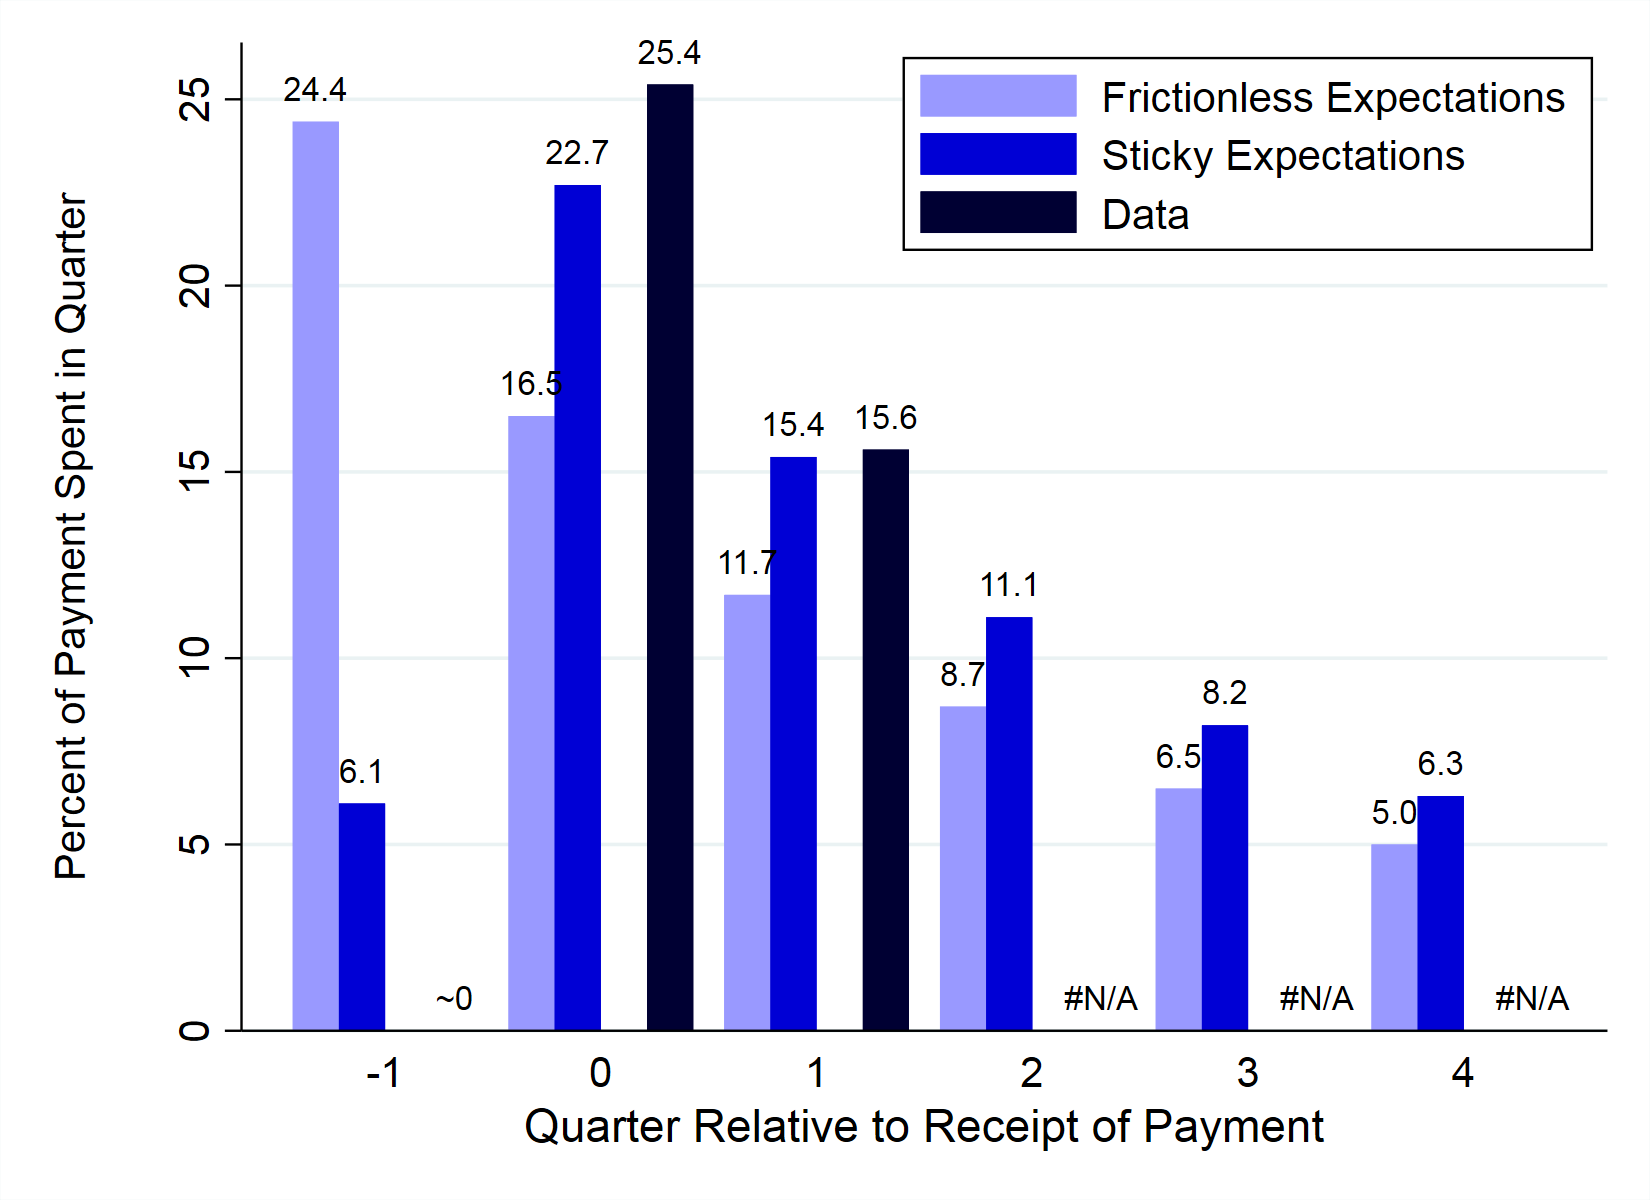
\includegraphics[width=1.0\textwidth]{./Figures/parkerExperiment}}

\begin{flushleft}
  \footnotesize Notes: The figure shows how consumption reacts to a fiscal stimulus payment in data and in models with frictionless and sticky expectations. The evidence from data is based on \cite{psjmMPC2008}, Table ~5 and \cite{brodaParker} (the lack of reaction of consumption in quarter $-1$, ``$\sim0$'' before the payment is received). To our knowledge, literature does not estimate the reaction in quarters 2 through 4, ``\#N/A''.
  \normalsize
  \end{flushleft}
\end{figure}

For this experiment, we employ a variant of our model that allows for ex-ante heterogeneity in households' discount factors, following \cite{cstwMPC}.\footnote{We also add unemployment insurance for this experiment.} By allowing for heterogeneity in the discount factor, we are able to calibrate the model to the distribution of wealth (and in particular the large fraction of the population with low levels of liquid wealth).  In keeping with related work by \cite{kvwWealthyH2m}, \cite{kmvHANK}, and others who emphasize the role of liquid assets, we calibrate the distribution of discount factors to match the empirical distribution of liquid wealth; \cite{cstwMPC} show that when their model is calibrated in that way, it generates an annual MPC of around 0.5.\footnote{This variant of the model produces similar results to our baseline model with respect to aggregate smoothness.\\
An alternative approach to calibrating the distribution of $\beta$ would be to target the distribution of MPCs by liquid wealth quantile, as reported for example by \cite{fhnMPC} or \cite{ckConsumption}. We also did this, but the results are too similar to the liquid wealth calibration to justify reporting.  We get similar (albeit lower) consumption responses when we calibrate the distribution of $\beta$ to match the distribution of net wealth.}

Our exact experiment is as follows.  An announcement is made in quarter $t-1$ that stimulus checks will arrive in consumers' bank accounts in period $t$.\footnote{This approximately fits the 2008 stimulus timetable. The announcement was made in February and the payments arrived between May and July. We also ran the experiment with two and three quarters advance notice and find the response on receipt of the payment remains in the right empirical range (19.9 and 16.7 percent respectively).} In line with our sticky expectation parameter, we assume 25 percent of households learn about the payment when it is announced, while the other three quarters of households are unaware until the payment arrives in period $t$. Furthermore, we assume the households who know about the upcoming payment are able to borrow against it in period $t-1$.

The experiment sharply differentiates the models with frictionless and sticky expectations both upon announcement of the payments and when households receive the payments (Figure~\ref{parker}). Upon announcement, consumption in the frictionless model substantially increases (households spend 24.4 percent of the payment), but under sticky expectations only one quarter of households update their beliefs when the announcement is made and consumption only rises by 6.1 percent of the stimulus payment.  This small effect is in line with \cite{brodaParker}, who estimate no economically or statistically significant change in spending when the household learns that it will receive a payment.  Instead, once the stimulus payment is received, sticky expectations households substantially increase their spending---by 22.7 percent of the payment, right in the middle of the 12--30 percent range estimated in \cite{psjmMPC2008}---as three quarters of them then learn about the payment by seeing it arrive in their bank account. In contrast, in the frictionless setup the reaction of spending upon the receipt of the payment is more muted (16.5 percent).\footnote{The identification method of \cite{psjmMPC2008} retrieves the difference between households who have received the payment and those who have not. In the sticky expectations model this is 14 percent of the payment, while it is zero in the frictionless model.} In the following two quarters, consumption in the sticky expectations model is higher by 15.4 and 11.1 percent of the payment amount respectively. This also fits with the empirical evidence suggesting around 40 percent of the stimulus payment is spent in the first three quarters (\cite{psjmMPC2008}).

The reader's intuition might have been that because our model exhibits little predictability in micro consumption growth when the consumer is experiencing ordinary income shocks (the $R^{2}$ of the predictive regression was only a few percent), and because it generates sluggishness in consumption with respect to aggregate shocks, the model would not be able to match the ample micro evidence showing high average MPCs, or the evidence from Parker and his coauthors showing that there is little ``anticipatory'' spending in advance of stimulus payments but a strong response to such payments once they have arrived.  This section shows that, in fact, the model is capable of matching the broad sweep of those micro facts, while continuing to match the aggregate excess smoothness facts.  The key is simple: In the version of our model calibrated to match high micro MPC's, people react robustly to shocks they know about, but they mostly don't know about the macro shocks until they see the money appear in their bank accounts.

 
\section{The Utility Costs of Sticky Expectations}\label{sec:uCost}

To this point, we have taken $\Pi$ to be exogenous (though reasonably calibrated).  Now, we ask what choices consumers would make if they could choose how much attention to pay in a framework where attention has costs.  Specifically, we imagine that newborns make a once-and-for-all choice of their idiosyncratic value of $\Pi$, yielding an intuitive approximating formula for the optimal updating frequency.\footnote{For a more thorough theoretical examination of the tradeoffs in a related model, see \cite{reis:inattentive}.}  We then conduct a numerical exercise to compute the cost of stickiness for our calibrated models.  The utility penalty of having $\Pi$ equal to our calibrated value of $0.25$, rather than updating every period ($\Pi=1$), are on the order of one two-thousandth of lifetime consumption, so that even small informational costs would justify updating aggregate information only occasionally.  Benefits of updating would be even smaller if the update yielded imperfect information about the true state of the macroeconomy; see below.

In the first period of life, we assume that the consumer is employed and experiences no transitory shocks, so that market resources are nonstochastically equal to $\mathsf{W}_t$; value can therefore be written as $\mathrm{v}(\mathsf{W}_t,\cdot)$.  There is no analytical expression for $\mathrm{v}$; but, fixing all parameters aside from the variance of the permanent aggregate shock, theoretical considerations suggest (and numerical experiments confirm) that the consequences of permanent uncertainty for value can be well approximated by:
\begin{eqnarray*}
   \mathrm{v}(\mathsf{W}_t,\cdot) & \approx & \grave{\mathrm{v}}(\mathsf{W}_t,\cdot) - \kappa \sigma^{2}_{\Psi}, \label{eq:vApprox}
\end{eqnarray*}
  where $\grave{\mathrm{v}}(\mathsf{W}_t,\cdot)$ is the value that would be generated by a model with no aggregate permanent shocks and $\kappa$ is a constant of approximation that captures the cost of aggregate permanent uncertainty (effectively, it is the coefficient on a first order Taylor expansion of the model around the point $\sigma_{\Psi}^{2}=0$).

Suppose now (again confirmed numerically---see Figure~\ref{costOfStickiness}) that the effect of sticky expectations is approximately to reduce value by an amount proportional to the inverse of the updating probability:

\begin{eqnarray}
  \label{eq:vBar}
   \widetilde{\mathrm{v}}(\mathsf{W}_t,\cdot) & \approx & \grave{\mathrm{v}}(\mathsf{W}_t,\cdot)-(\kappa/\Pi)\sigma^{2}_{\Psi} \label{eq:vApproxSticky}
\end{eqnarray}
 
This assumption has appropriate scaling properties in three senses:
\begin{itemize}
\item If $\sigma^{2}_{\Psi}=0$ so that there are no permanent shocks, then
the cost of stickiness is zero (given our assumption that initial perceptions are correct).
\item If the probability of updating is $\Pi=1$ so that perceptions
are always accurate, value is the same as in the frictionless model.
\item If expectations never adjust, then $\Pi=0$ and the utility cost of stickiness is infinite,
which is appropriate because consumers would be making choices based on
expectations that would eventually be arbitrarily far from the truth.
\end{itemize}

Now imagine that newborns make a once-and-for-all choice of the value of $\Pi$; a higher $\Pi$ (faster updating) is assumed to have a linear cost $\iota$ in units of normalized value.\footnote{Think of this as utility costs of paying attention to macroeconomic news instead of, say, sports news or other more pleasurable news items; since we are examining a model that has been normalized by productivity, this could alternatively be loosely interpreted as a time cost of gathering information.}  The newborn's objective is therefore to choose the $\Pi$ that solves:
\begin{eqnarray*}
   \max_{\Pi} ~ \grave{\mathrm{v}}(\mathsf{W}_t,\cdot)-(\kappa/\Pi)\sigma^{2}_{\Psi}-\iota\Pi. \label{eq:pickPi}
\end{eqnarray*}
 The first order condition is:
\begin{eqnarray*}
     0 & = & \Pi^{-2}\kappa\sigma^{2}_{\Psi}-\iota,
\\  \Pi^{2} & = & (\kappa \sigma^{2}_{\Psi})/\iota,
\end{eqnarray*}
which leads to the conclusion that the consumer will
pick the $\Pi$ satisfying:
\begin{eqnarray*}
  \Pi & = &  (\kappa/\iota)^{0.5} \sigma_{\Psi}. \label{eq:bestPi}
\end{eqnarray*}
 

\begin{figure}
  \centering
\caption{Costs of Stickiness $\omega$ and Probability of Aggregate Information Updating $\Pi$}
\label{costOfStickiness}
{ 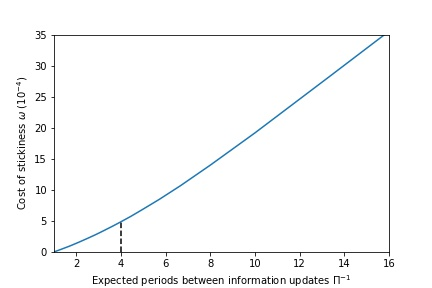
\includegraphics[width=1.0\textwidth]{./Figures/uCostvsPiInv}}

\footnotesize Notes: The figure shows how the utility costs of updating $\omega$ depend on the probability of updating of aggregate information $\Pi$ in the SOE model.
\end{figure}

Thus, the speed of updating should be related directly to the utility cost of permanent uncertainty $(\kappa)$, inversely to the cost of information (cheaper information induces faster updating), and linearly to the standard deviation of permanent aggregate shocks.

Our calibrated models can be used to numerically calculate the welfare loss from our specification of sticky expectations as an agent's willingness to pay at birth in order to avoid having $\Pi=0.25$ for his entire lifetime.\footnote{Additional numeric details of the cost of stickiness calculation can be found in online Appendix~\ref{appendix:uCost}.}  Specifically, we calculate the percentage loss of permanent income that would make a newborn indifferent between living in the world with $\Pi=0.25$, or living in a frictionless world after paying the cost of abolishing the friction.\footnote{The measure of the cost of stickiness we report is almost surely larger than the willingness to pay of an agent at a \textit{random period of life}.  As newborns do not yet have a buffer stock and are on the steeper portion of their consumption function than they will generally find themselves, consumption errors from sticky expectations are larger in the first few periods of life, and so the utility costs of stickiness are somewhat front-loaded.}

Using notation from the theoretical exercise above, define a newborn's average lifetime (normalized) value at birth under frictionless and sticky expectations as respectively:
\begin{equation*}
\overline{\mathrm{v}}_0 \equiv \Ex \big[ \mathrm{v}(\mathsf{W}_t,\cdot)\big], \qquad \overline{\widetilde{\mathrm{v}}}_0 \equiv \Ex \big[ \widetilde{\mathrm{v}}(\mathsf{W}_t,\cdot)\big],
\end{equation*}
where the expectation is taken over the distribution of state variables other than $m_{t,i}$ that an agent might be born into.  We compute these quantities by averaging the discounted sum of consumption utilities experienced by households over their simulated lifetimes.  A newborn's willingness to pay (as a fraction of permanent income) to avoid having sticky expectations can then be calculated as:
\begin{eqnarray}\label{eq:WTP}
\omega & = & 1 - \bigg(\,\frac{\overline{\widetilde{\mathrm{v}}}_0}{\overline{\mathrm{v}}_0} \bigg)^{\frac{1}{1-\rho}}.
\end{eqnarray}

A newborn in our model is willing to give up about 0.05 percent of his permanent income to remain frictionless.  These values are comparable to the findings of \cite{mackWiedREStud15}, who construct a model in which, as in \cite{reis:inattentive}, agents optimally choose how much attention to pay to economic shocks by weighing off costs and benefits.  They find (p.\ 1519) that the cost of suboptimal tracking of aggregate shocks is 0.06 percent of steady state consumption.\footnote{The theme goes back at least to \cite{cochrane_nearRational}.}

Now that we have explained how to compute the cost of stickiness numerically, we can test our supposition in equation \eqref{eq:vApproxSticky} that the cost of stickiness might have a roughly inverse linear relationship to $\Pi$.  Figure~\ref{costOfStickiness} plots numerically computed willingness-to-pay $\omega$ for various values of $\Pi^{-1}$; the relationship is close to linear, as we speculated.

Our preferred interpretation is not that households deliberately choose $\Pi$ optimally due to a cost of updating, but instead that $\Pi$ is exogenous and represents the speed with which macroeconomic news arrives ``for free'' from the news media.  This could explain why the parameter $0.25$ seems to work about equally well for inflation, unemployment expectations, and consumption -- all of them are informed by the same flow of free information. An objection to this interpretation is that a household who has not updated for several years would face a substantially larger loss from continuing to be oblivious and would eventually feel the need to deliberately look up some aggregate facts.  At the cost of a large computational and theoretical investment, we could modify the model to allow consumers to behave in this way, but it seems clear that the {\it ex ante} benefit would be extremely small, because the likelihood of being sufficiently out of date to make costly mistakes is negligible.  Intuitively, we can calculate that at any given moment, only 3 percent of households will have information that is more than 3 years out of date ($(1-\Pi)^{12} \approx 0.03$), of households will be in this position.  Furthermore, simple calculations show that if we change the simulations so that households always exogenously update after three years, this barely changes aggregate dynamics (the estimate of $\chi$ slightly increases from 0.660 to 0.667 in the small open economy model).

\section{Muth--Lucas--Pischke and \cite{reis:inattentive}} \label{sec:Comparisons}

Now that our calibrations and results have been presented, we are in position to make some quantitative comparisons of our model to two principal alternatives to habit formation (or our model) for explaining excess smoothness in consumption growth, by Pischke and by Reis.

\subsection{Muth--Lucas--Pischke}
The longest-standing rival to habit formation as an explanation of consumption sluggishness is what we will call the Muth--Lucas--Pischke (henceforth, MLP) framework.  The idea is not that agents are inattentive, but instead that they have imperfect information on which they perform an optimal signal extraction problem.

\cite{muthOptimal}'s agents could observe only the level of their income, but not the split between its permanent and transitory components.  He derived the optimal (mean-squared-error-minimizing) method for estimating the level of permanent income from the observed signal about the level of actual income.  \cite{lucas:imperfectInfo} applied the same mathematical toolkit to solve a model in which firms are assumed to be unable to distinguish idiosyncratic from aggregate shocks.  \cite{pischkeMicroMacro} combines the ideas of Muth and Lucas and applies the result to micro consumption data: His consumers have no ability at all to perceive whether income shocks that hit them are aggregate or idiosyncratic, transitory or permanent.  They see only their income, and perform signal extraction on it.

Pischke calibrates his model with micro data in which he calculates that transitory shocks vastly outweigh permanent shocks.\footnote{Pischke's estimates constructed from the {\it Survey of Income and Program Participation} are rather different from the magnitudes of transitory and permanent shocks estimated in the extensive literature---mostly subsequent to Pischke's paper---cited in our calibration section above.}  So, when a shock arrives, consumers always interpret it as being almost entirely transitory and change their consumption by little.  However, macroeconometricians have long known that {\it aggregate} income shocks are close to permanent.  When an aggregate permanent shock comes along, Pischkian consumers spend very little of it, confounding the aggregate permanent shock's effect on their income with the mainly transitory idiosyncratic shocks that account for most of the total variation in their income.  This misperception causes sluggishness in {\it aggregate} consumption dynamics in response to aggregate shocks.

In its assumption that consumers fail to perceive aggregate shocks immediately and fully, Pischke's model resembles ours.  However, few papers in the subsequent literature have followed Pischke in making the assumption that households have no idea, when an idiosyncratic income shock occurs, whether it is transitory or permanent.  Especially in the last decade or so, the literature instead has almost always assumed that consumers can perfectly perceive the transitory and permanent components of their income; \hyperlink{Why-Consumers-See-Individual-Shocks}{see our defense of this assumption above}.

Granting our choice to assume that consumers correctly perceive the events that are idiosyncratic to them (job changes, lottery winnings, etc), there is still a potential role for application of the MLP framework:  Instead of assuming sticky expectations, we could instead have assumed that consumers perform a signal extraction exercise on \textit{only} the aggregate component of their income, because they cannot perceive the transitory/permanent split for the (tiny) part of their income change that reflects aggregate macroeconomic developments.

In principle, such confusion could generate excess smoothness; for a detailed description of the mechanism, \hyperlink{MuthLucasPischke}{see} online Appendix~\ref{appendix:Muth}.  But, defining the signal-to-noise ratio $\varphi=\sigma^2_{\Psi}/\sigma^2_{\Theta}$, Muth's derivations imply that the optimal updating coefficient is:
  \begin{eqnarray}
\Pi & = & \varphi \sqrt{1+\varphi^{2}/4} - (1/2) \varphi^{2} \label{eq:muthOptimal}
  \end{eqnarray}
Plugging our calibrations of $\sigma^2_{\Psi}$ and $\sigma^2_{\Theta}$ from section \ref{sec:calibration} into \eqref{eq:muthOptimal}, the model yields a predicted value of \ifthenelse{\boolean{false}}{$1-\Pi \approx 0.17$}{$(1-\Pi) \approx 0.17 $}---very far below the approximately $0.6$ estimate from \cite{hrsHabit} and even farther below our estimate of roughly $0.7$--$0.8$ for U.S.\ data.  This reflects the well-known fact that aggregate income is hard to distinguish from a random walk; if it were perceived to be a perfect random walk with no transitory component at all, the serial correlation in its growth would be zero.  So, in practice, allowing signal extraction with respect to the aggregate data is not a path to explaining excess smoothness.

\subsection{\cite{reis:inattentive}}

Leaving aside our earlier criticisms of its fidelity to microeconomic evidence, the model of \cite{reis:inattentive} has a further disadvantage relative to any of the other three stories (habits, MLP, or our model) with respect to aggregate dynamics. In Reis's model consumers update their information on a regular schedule---under a plausible calibration of the model, once a year. One implication of the model is that the change in consumption at the next reset is unpredictable; this implies that aggregate consumption growth would be unpredictable at any horizon beyond, say, a year.\footnote{In contrast, our model exhibits significant predictability beyond one year. The value of $\chi$ in the `horse-race' regression for the SOE economy is 0.66 when the right hand side is lagged by one quarter (see Table~\ref{tPESOEsim}). Adding an extra one and two years' lag to the right hand side sees $\chi$ decline approximately as an AR(1), to 0.20 and 0.06 respectively.}  But, business cycle analysts felt compelled to incorporate sluggishness into macroeconomic models in large part to explain the fact that consumption growth is forecastable over extended periods---empirical impulse response functions indicate that a macroeconomically substantial component of the adjustment to shocks takes place well beyond the one year horizon.  A calibration of the Reis model in which consumers update once a year therefore fails to solve a large part of the original problem (of medium-term predictability).

 

\section{Conclusion} \label{sec:Conclusion}

Using a traditional utility function that does not incorporate habits, the literature on the microfoundations of consumption behavior has made great strides over the past couple of decades in constructing models that are faithful to many of the microeconomic facts about consumption, income dynamics, and the distribution of wealth.  But over roughly the same interval, habit formation has gone from an exotic hypothesis to a standard assumption in the representative agent macroeconomics literature, because habits allow representative agent models to match the measured smoothness in aggregate consumption growth that is of practical importance in quantitative macroeconomic dynamics.  This conflict, thrown into sharp focus by the recent meta-analysis of both literatures by \cite{hrsHabit}, is arguably the most important puzzle in the microfoundations of macroeconomic consumption dynamics.

We show that this conflict can be resolved by applying insights from the literature on `inattention' that has developed robustly since the early contributions of \cite{simsInattention}, \cite{woodfordImperfect}, \cite{mrSlumps}, and others.  In the presence of such inattention, aggregation of the behavior of microeconomic consumers without habits generates aggregate consumption dynamics that match the `excess smoothness' facts that have induced the representative agent literature to embrace habits.

The sticky expectations assumption is actually more attractive for modeling consumption than for other areas where it has been more widely applied, because in the consumption context there is a well-defined utility-based metric for calculating the cost of sticky expectations.  This is in contrast with, say, models in which households' inflation expectations are sticky; the welfare cost of misperceiving the inflation rate in those models is typically harder to quantify.  The cost to consumers of our proposed degree of macroeconomic inattention is quite modest, for reasons that will be familiar to anyone who has worked with both micro and macro data: Idiosyncratic variation is vastly greater than aggregate variation.  This means that the small imperfections in macroeconomic perceptions proposed here have very modest utility consequences.  So long as consumers respond appropriately to their idiosyncratic shocks (which we assume they do), the failure to keep completely up-to-date with aggregate developments simply does not matter much.

While a number of previous papers have proffered the idea that inattention (or imperfect information) might generate excess smoothness, the modeling question is a quantitative one (`how much excess smoothness can a sensible model explain?').  We argue that the imperfect information models and mechanisms proposed in the prior literature are quantitatively unable simultaneously to match the micro and macro quantitative facts, while our model matches the main stylized facts from both literatures.

In future work, it would be interesting to enrich the model so that it has plausible implications for how the degree of attention might vary over time or across people, and to connect the model to the available expectations data---for example, measures of consumer sentiment, or measures of uncertainty constructed from news sources, cf \cite{bbdUncertainty}.  Such work might be particularly useful in any attempt to understand how behavioral dynamics change between normal times in which news coverage of macroeconomic dynamics is not front-page material versus crisis times, when it {\it is}.

\processdelayedfloats

\small
\bibliography{cAndCwithStickyE}
\normalsize

\end{document}
